\begin{flushright}

\end{flushright}\section{Performance Evaluation}
\label{sec_perf}
 

\subsection{Simulator Overview}
To evaluate the performance and power consumption of the proposed
architecture, we simulate the multi-core heterogeneous architecture
by extending Multi2Sim - a superscalar, multithreaded and multicore
simulator - with a reconfigurable accelerator unit. 
 The specification of our simulated architecture is shown in Table
\ref{tbl_parameters}. The processor core technology and operating
frequency are modeled based on the Atom 330 processor. We set the
number of cores to be eight in the baseline configuration. Afterwards, we vary the
number of cores to explore the area allocation to the accelerators as well as the cores. 
The ICAP interface runs at 100 MHz, although over-clocking ICAP is
possible in practice \cite{Hansen:2011dt}.

\begin{table}
\scriptsize
\begin{center}
  \begin{tabular} { | l | l | }
    \hline
    \textbf{Item} & \textbf{Parameter} \\
    \hline
    \hline
	Core & 8 \\
	\hline
	Core Spec & 45nm @ 1.6 GHz \\
	\hline
	Accelerator Spec & 45nm @ 200 MHz \\
	\hline
	ICAP & 32 bit bus width @ 100 MHz \\
	\hline
	L1 Instr/Data \$ Size (KB) & 32 \\
	\hline
    L1 Instr/Data \$ Associativity & 4\\
    \hline
    L1 Instr/Data \$ Block Size (Bits) & 64\\
    \hline
    L1 Instr/Data \$ Number of Sets & 128\\
    \hline
    L1 Instr/Data \$ Latency (Cycles) & 3 \\
   	\hline
   	L2 Cache Size (MB) & 4 (shared) \\
   	\hline
    L2 Associativity & 8\\
    \hline
    L2 Block Size (Bits) & 512\\
    \hline
    L2 Number of Sets & 1024 \\
    \hline
    L2 Latency (Cycles) & 20\\
    \hline
    CPU Cache Coherence & MOESI\\
    \hline
    Accelerator Data Buffer Size (KB) & 8 \\
    \hline
    Accelerator Data Buffer Coherence & MOESI\\
    \hline
    Memory Size (GB) & 8 \\
    \hline
    Memory Latency (Cycles) & 200 \\
    \hline
    Memory Data Block Size (Bytes) & 512\\
    \hline
    Memory Page Size (Bytes) & 8192\\
    \hline
    Memory Replacement Policy & Pseudo LRU\\
    \hline
    Network Topology & 2-D Mesh\\
    \hline
    Network Bandwidth (MB/s) & 1024\\
    \hline
  \end{tabular}
\caption{Hardware Specification}
\label{tbl_parameters}
\end{center}
\end{table}


To model the profiling and scheduling overheads within the simulations,
we evaluate the overhead of the profiler in the wrapper function and the
three scheduling methods: na\"{\i}ve, bandwidth-first, or speedup-first. For
the worst case, the profiler and the wrapper function's overhead takes up
to 0.017 \% per profiling window.  The worst case occurs only
when the reconfiguration controller accepts the current acceleration
request within the profiling window. The two knapsack combination
scheduling algorithms introduce more overhead than the na\"{\i}ve scheduling. However, further evaluation shows that the overhead of both the bandwidth-first and the speedup-first algorithms introduce a neglectable overhead of 0.130 \% per profiling window. 

\subsection{Benchmarks}
We use all eight acceleration functions from the
open-source accelerator store \cite{accstore} to build a synthetic
workload that simulates the dynamic workloads within cloud and mobile
environments.  In this case, we defer using real-world cloud applications to our
future work.  These applications cover a wide range of areas
including encryption/decryption ({\em 3DES} \cite{openssl}), numerical
calculation ({\em Jacobi} \cite{jacobi-wiki}), vision and navigation
({\em SLAM-C and SLAM-J} \cite{openslam}), feature detection ({\em SURF} and
{\em IDSI} \cite{opencv}), image processing ({\em Segmentation}
\cite{segmentation-wiki}) and bioinformatics ({\em Smith-Waterman}
\cite{smithwaterman-wiki}). Moreover, the aforementioned software applications have
corresponding accelerator implementations which provide
performance as well as area allocation details. Minor modifications were done in order to generate the
final benchmark mixture, including preparing the input data set for
each function as well as the creation of multiple threads.

To emulate the dynamics of workload arrival, we model the inter-arrival time between
each benchmark as a Poisson distribution. The average
inter-arrival time is set to 500 million cycles, 312.5 ms
in real time if the system is running at 1.6 GHz, which in turn is close to the
cycle time of one iteration for our shortest benchmark IDSI. We compare
the Poisson arrival pattern with the default pattern of continuous
arrival, where the inter-arrival time is zero.

\subsection{Modeling Accelerators}
As there is no accelerator modeled in the stock Multi2Sim simulator,
 a general purpose core is modified to simulate a reconfigurable
accelerator unit. A best effort is made to model the
computation, the memory access, along with the reconfiguration delays based
upon prior work as well as our own benchmark studies. 

We model the timing of each accelerator by using their different
speedup values reported in the prior work as listed in Table
\ref{tbl_benchmark}. The speedup numbers are scaled to the 
operating frequencies for each core core as well as the reconfigurable logic used in our
simulations. 

We are interested in understanding the memory access
patterns, specifically the footprint, the data size and the frequency.  Furthermore, we are interested in modeling
the patterns within the accelerators using a series of high fidelity simulations. Towards this end, we profile the memory
activities by logging the memory access traces for each 
acceleration function.
Figure \ref{fig_mem_access} illustrates the memory access pattern for
two benchmark applications: Jacobi and SLAM-J. The horizontal axis represents
the time of the access, while the vertical axis represents the address within a given 
page range. In this way, we observe the temporal and spatial
characteristics of the memory accesses. It can be seen that {\em
  Jacobi} has larger number of accesses and that the
accesses span a wider address range. We model similar memory
access patterns when simulating the accelerators.  In addition, we visually
differentiate memory bound applications from computationally intensive
applications. 

The overhead of a DMA transfer is modeled within the approximation
formula derived from \cite{Saidi:2012}: $ T(s) = I + \alpha \times b \times
s$, where $I$ is the fixed initial cost, which includes issuing commands
along with the TLB translation, $\alpha$ is the transfer cost rate in
$cycles/byte$, $b$ is the basic block size, and $s$ is the super block
size. Given that the DMA command along with the TLB translation are already modeled separately within the wrapper libraries and
the stock Multi2Sim simulator, $I$ is set to 0 in this case. We choose $\alpha$
to be 2 cycles/byte as an average number \cite{Saidi:2012}. The variables $b$ and $s$
are to be determined by the appropriately relevant functions.


\begin{figure}
    \centering
    \includegraphics[width=6.0in]{Mem-Access}
	\caption{Memory access pattern of Jacobi (left) and SLAM-J (right)}
\label{fig_mem_access}
\end{figure}


The IO buffers on each of the accelerators are modeled by
modifying the Multi2Sim cache models. In this case, the MOESI cache coherence
protocol remains effective. The TLBs are employed to handle the virtual memory
address translation.  We have studied the impact of the size of the IO
buffers on the performance of the {\em Transformer}'s reconfigurable
logic. The results, which are not depicted here, reveal that the performance of
the accelerator increases significantly from 8KB to 32KB, beyond which no
substantial improvement is observed. As a result, our simulations use 32KB as
the default buffer size.

The partial reconfiguration delay $T_R$ is modeled as $ T_R = \frac{S_{pbs}}{ B_{ICAP} / C_{ICAP}} $,
where $S_{pbs}$ is the size of
partial bitstream, and $B_{ICAP}$ and $C_{ICAP}$ are the bus bandwidth
as well as the cycle time for ICAP.
Since the partial reconfiguration time depends on the size of the partial bit
stream, we conservatively model the reconfiguration time using the
largest bitstream size observed amongst all of the benchmarks within our simulations. 


\subsection{Power Model}
The dynamic and static power consumption of the general purpose cores are
estimated by using HP McPat v0.8 \cite{mcpat}. The power consumption of the reconfigurable logic
is modeled as follows. We track the number of
logic elements used by the accelerator functions at run time, 
including the number SLICE, FF, DSP48, and BRAM elements. The number of each logic element type serves as the input data to the 
Xilinx Power Estimator
\cite{xpe}, which serves to calculate the reconfigurable logic's power consumption.  
We scale the power of the reconfigurable logic to the 45 nm technology scale
so that both the cores and the accelerators are at the same technology
level. The total power consumption is the sum of the power of
the reconfigurable logic as well as the power reported by McPat for each of the
cores. 


\subsection{Simulation Results}
\label{sec_simu_result}

\subsubsection{Speedup of Multiple Copies of a Single Workload}

We first study the effectiveness of the {\em Transformer} on single function 
workloads. A software thread repeatedly executes a single function, such as the 3DES function,
 and then we gradually increase the number of threads. In this setting, both 
scheduling methods will select the same accelerator since the wrapper function
intercepts only one kind of library call. As a result, we only compare the architectures with
or without accelerators. 
Figure \ref{fig_num_of_apps} displays the performance speedup on the y
axis while the x axis displays the number of threads. The
baseline performance is the execution time for the $k$ threads on a multicore
architecture without an accelerator. We 
observe that the speedup for the 3DES function is significant, $\sim14\times$, when the number of threads is
approximately two, beyond which the speedup decreases. In this case the
resources available within the accelerator logic only allows up to two
3DES accelerator functions to be instantiated. The remaining threads
are executed as software within the cores.  As a result, the level of speedup is not
as significant as the ones observed within the earlier cases.  Other functions
experience similar trends but the number of acceleration function
copies differs from benchmark to benchmark.   

The disparity in the reconfigurable resource requirements among benchmarks
validates the observed opportunities for combining accelerators. Further
analysis indicates that the 3DES accelerator function requires 40\% of 
the BRAM resources of the reconfigurable logic, so that only two copies of
3DES functions can be instantiated. However, other types of
resources such as the LUT remain abundant when accommodating
functions such as SLAM-C, which requires only 9.2\% of the LUTs and none of the
BRAMs. Below, we illustrate the run-time accelerator instantiation and combination within Figure
\ref{fig_acc_timeline}.   

\begin{figure}
    \centering
    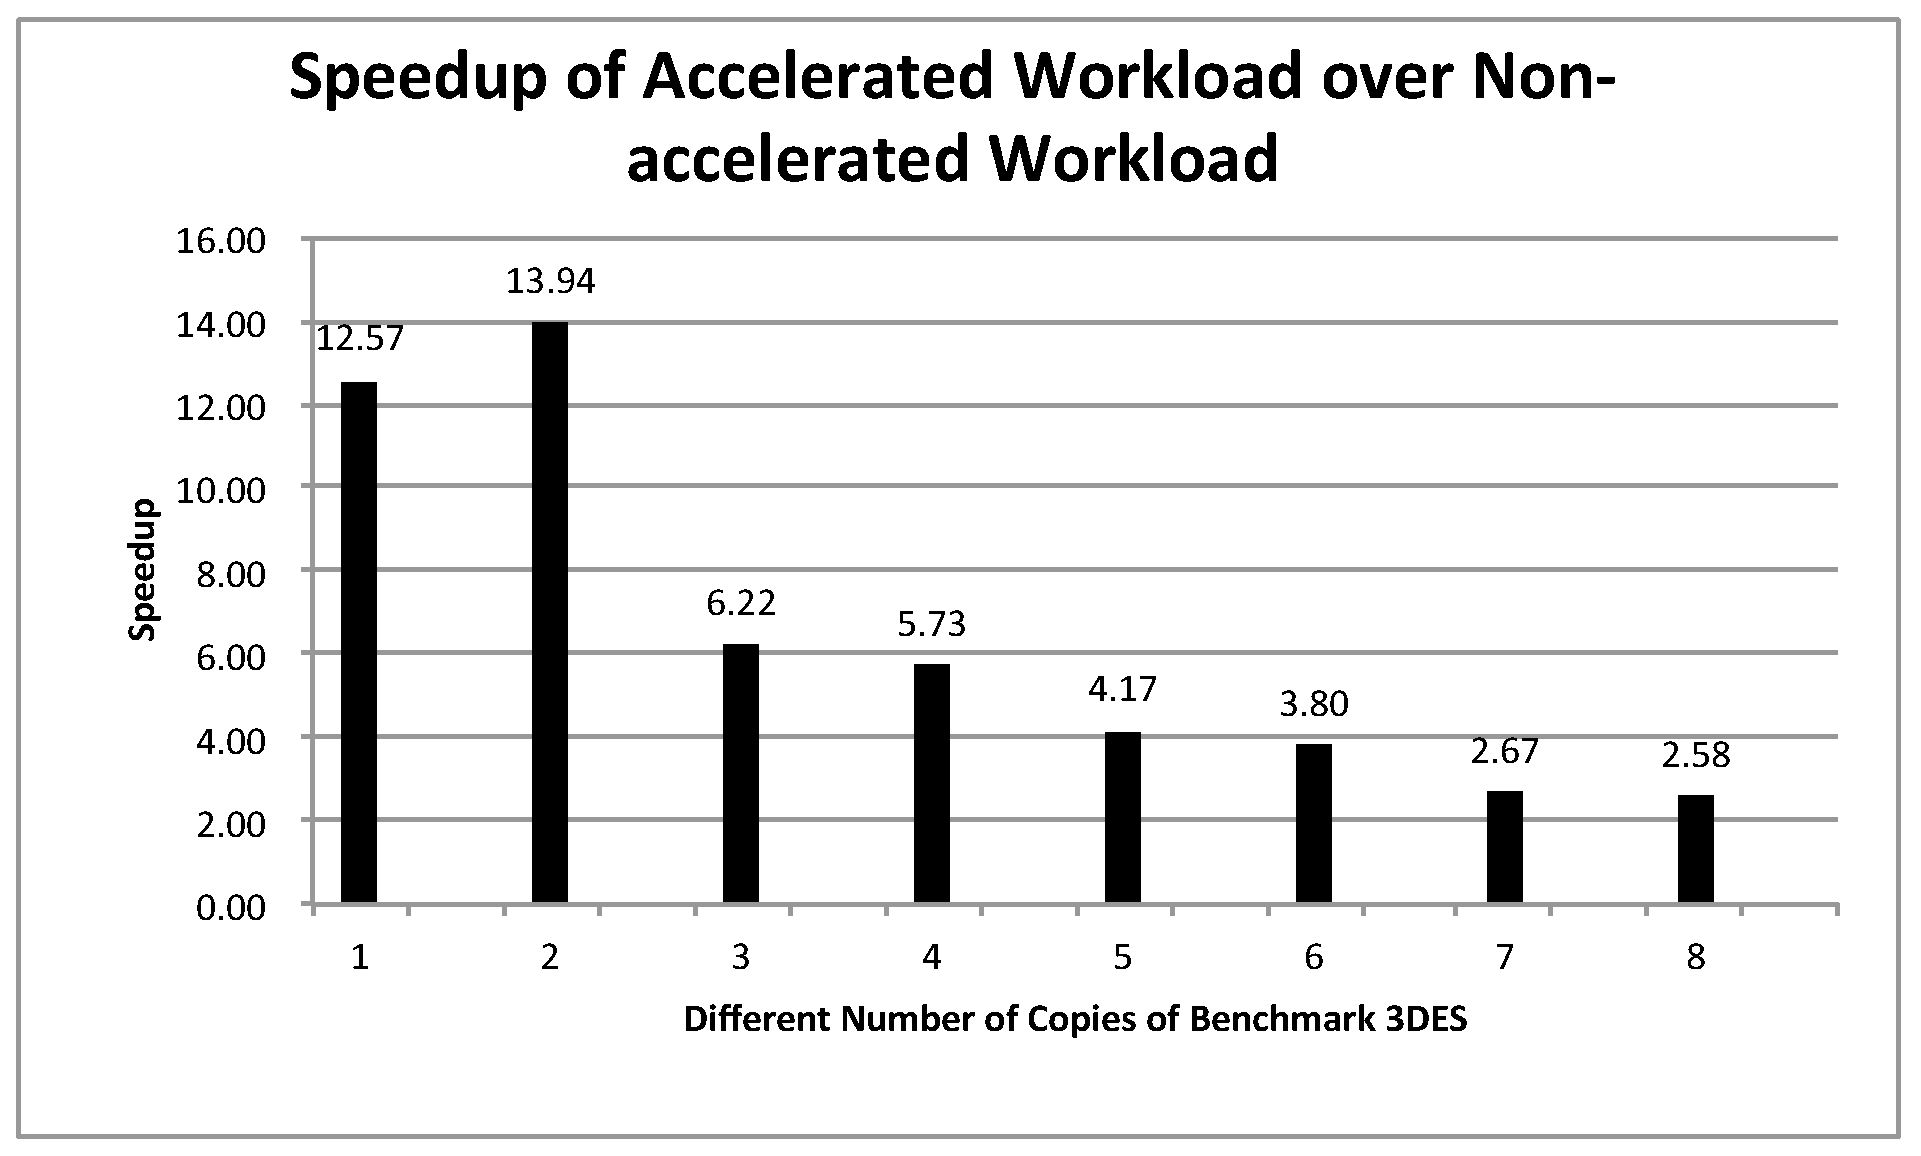
\includegraphics[width=4.5in]{Increase-Num-of-Apps}
    \caption{Speedup of Multiple Copies of a Single Workload Type}
    \label{fig_num_of_apps}
\end{figure}

\subsubsection{Speedup and Energy Efficiency of Workload Mixtures}

Given a mixture of the workloads, the instantiation of accelerator
functions is subject to the run-time demands as well as the constraints of the logic resources.
 We execute the synthetic workloads on the {\em Transformer} with eight
cores and one reconfigurable logic unit, which in this case matches the size of one Xilinx
Spartan 3E FPGA. The workload's arrival either follows a Poisson distribution or
a continuous back-to-back distribution. We issue 100 thousand billion instructions of
the benchmark bundle and record the number of completed functions as well as the
cycle times. 

\begin{figure}
    \centering
    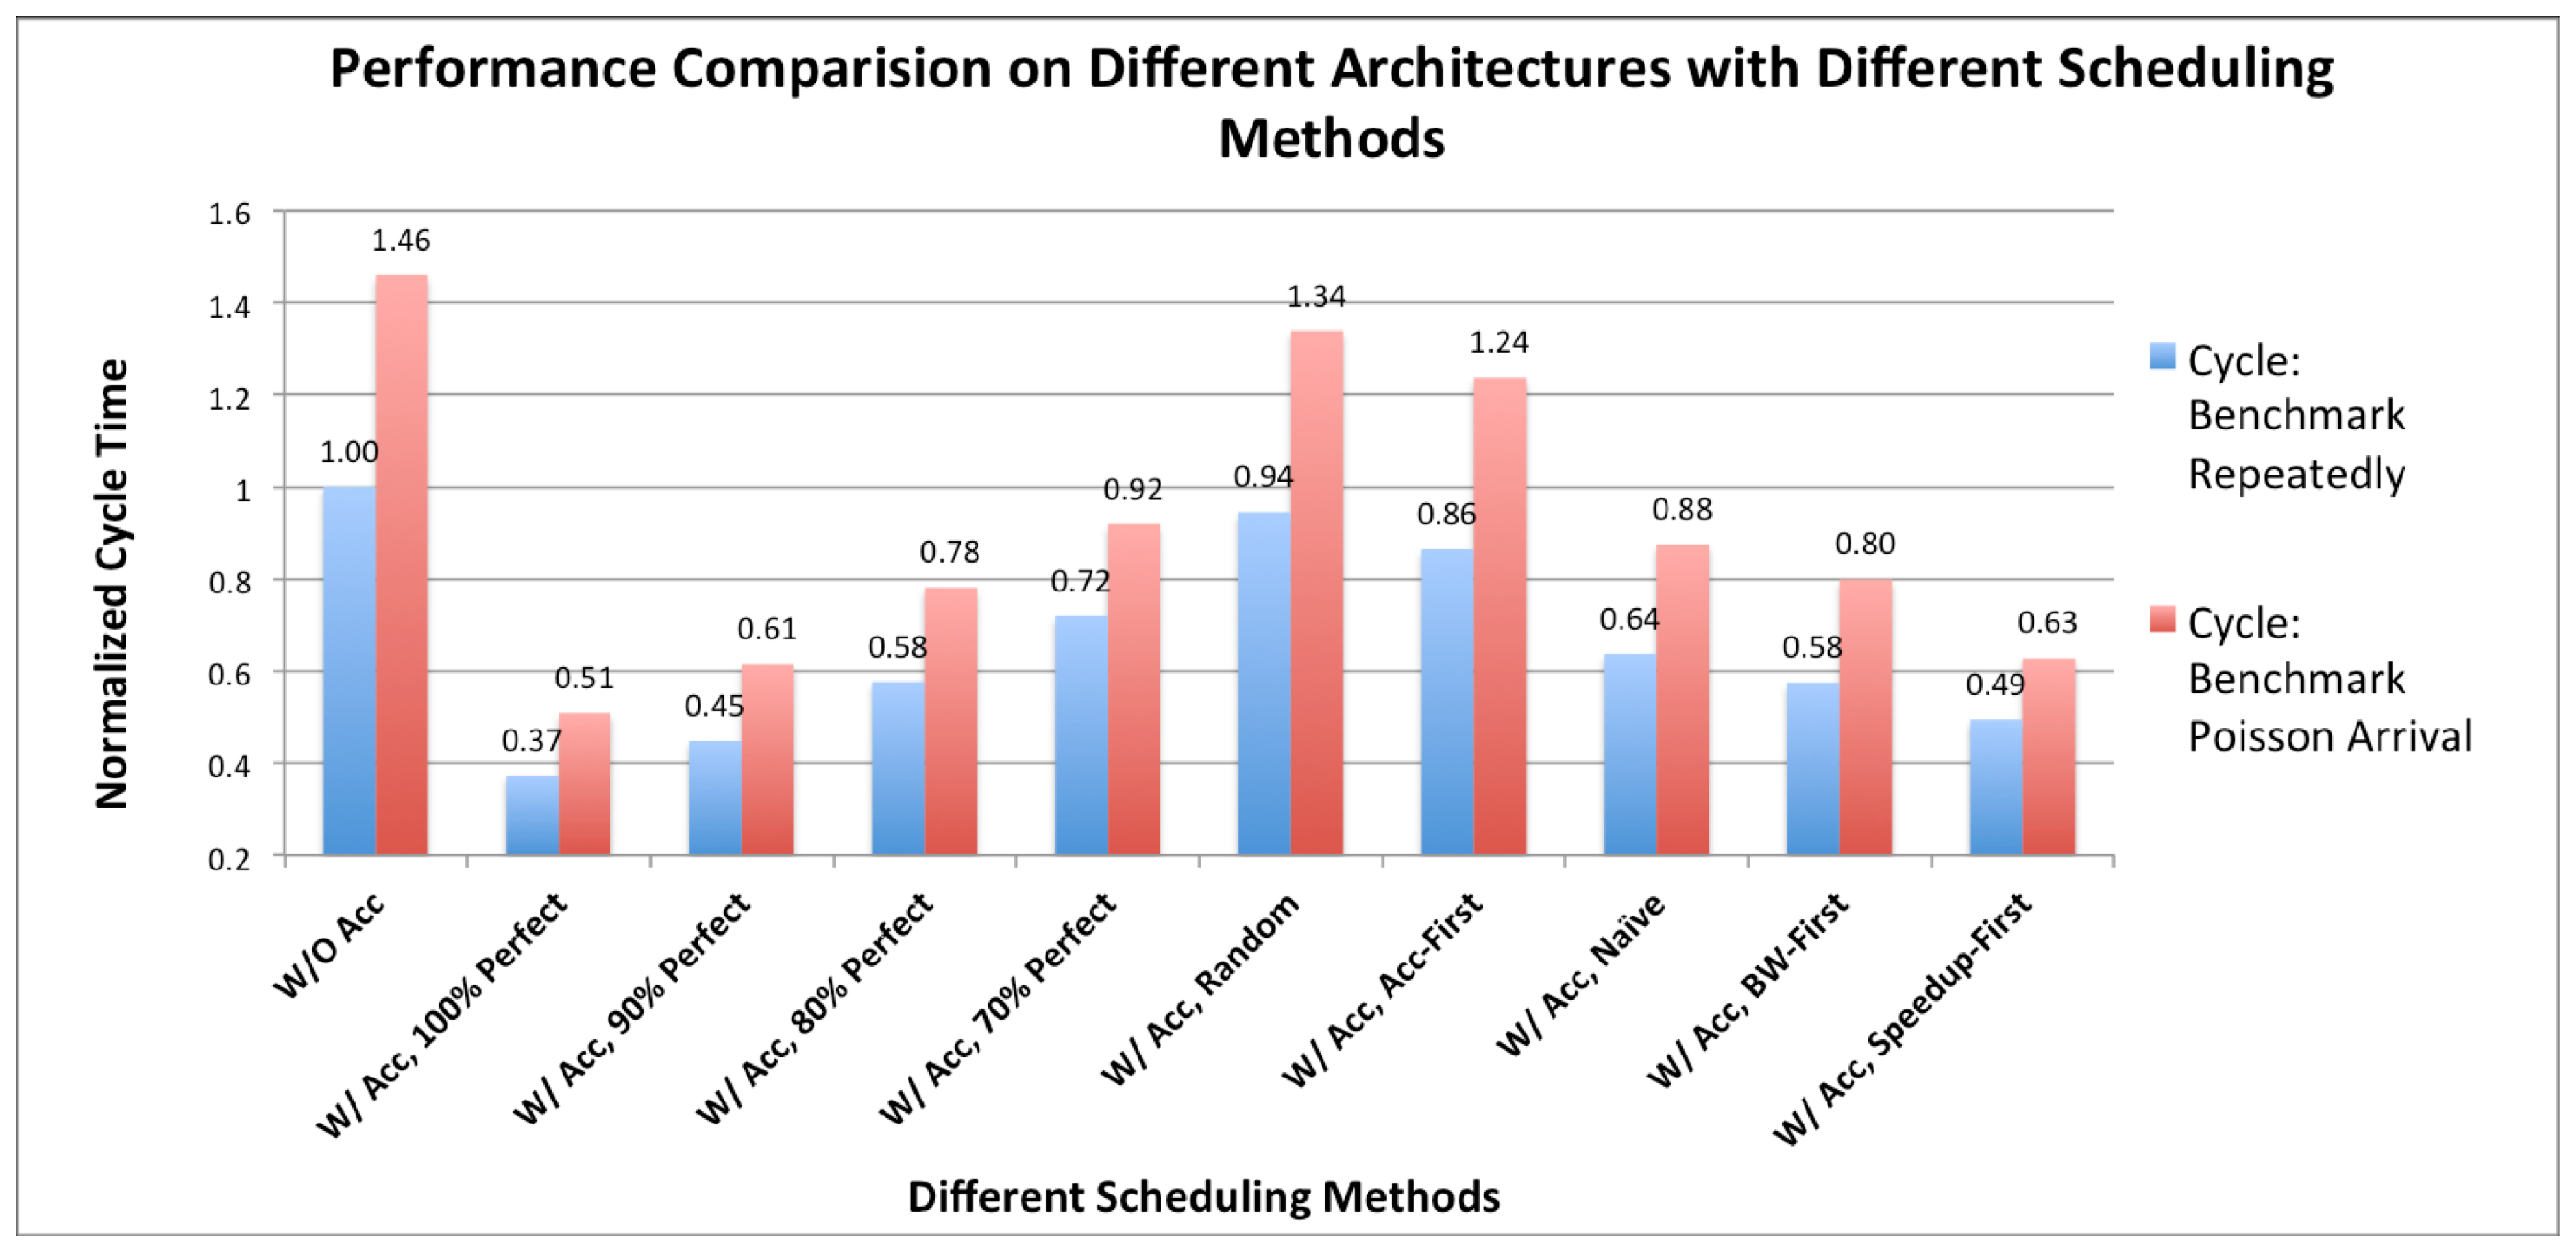
\includegraphics[width=4.5in]{Cycle-8core}
    \caption{Performance Comparison of Accelerated Architecture and Scheduling Algorithms}
    \label{fig_8core_cycle}
\end{figure}

\begin{figure}
    \centering
    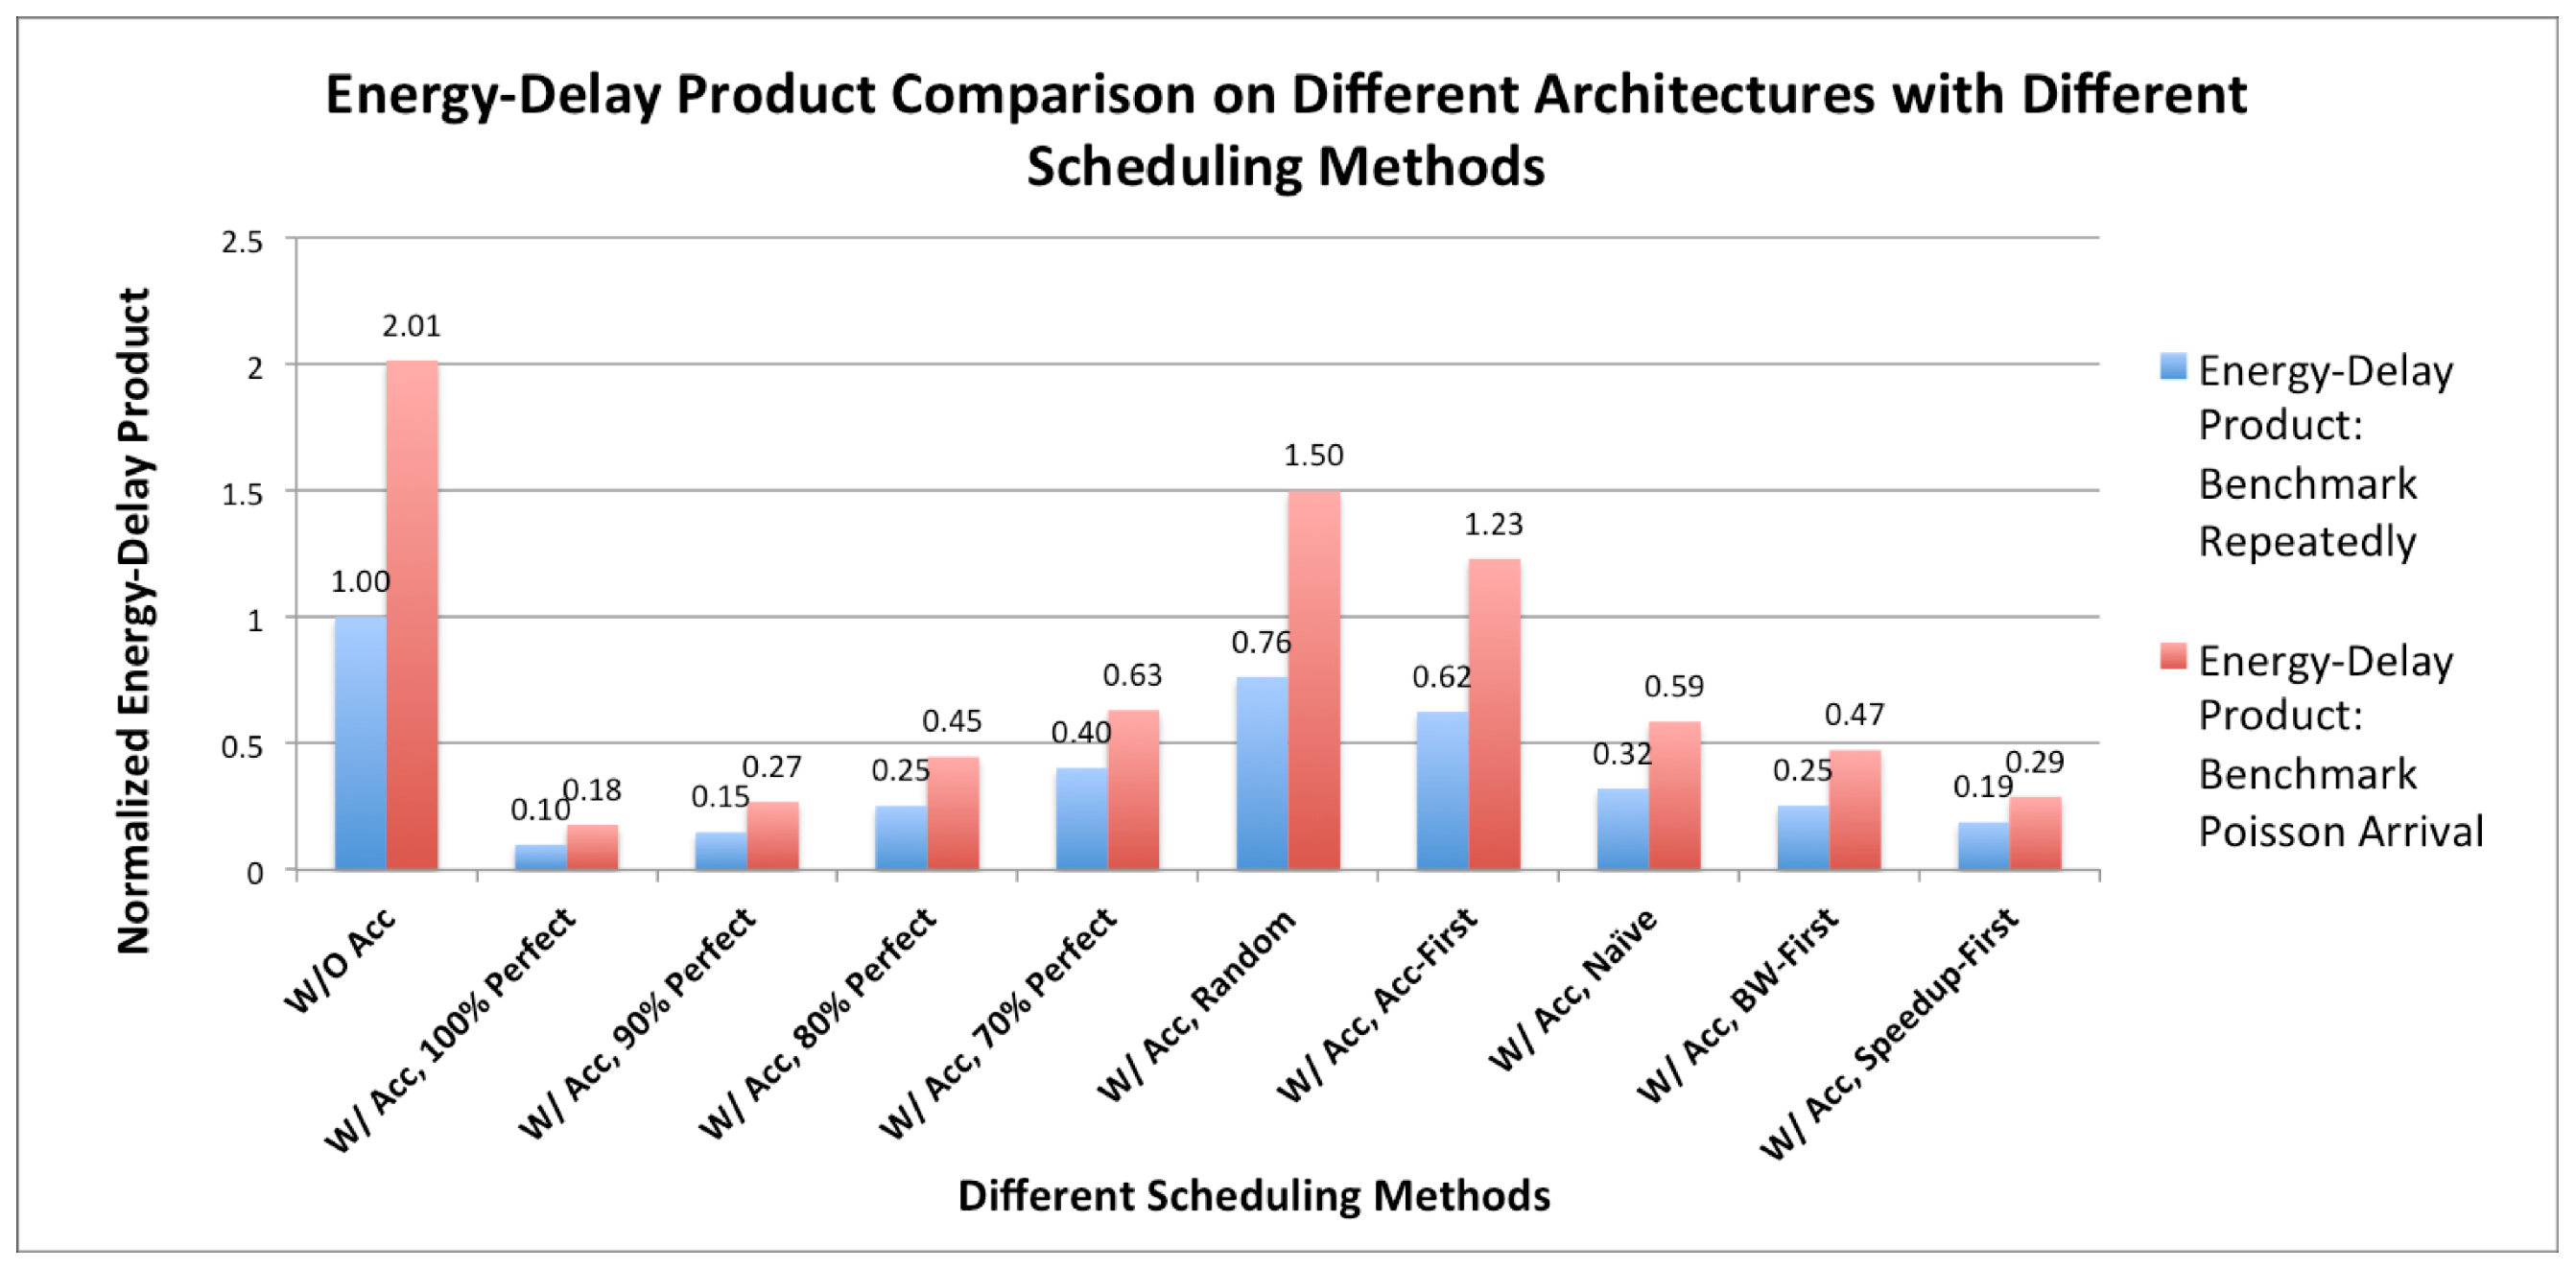
\includegraphics[width=4.5in]{Energy-Delay-8core}
    \caption{Energy-delay Product Comparison}
    \label{fig_8core_energy_delay}
\end{figure}

Figure \ref{fig_8core_cycle} depicts the performance of different
scheduling methods. The x-axis denotes different
architectures as well as scheduling methods, including:
 no accelerator, ``W/O Acc",
 with the accelerator and 100\% perfect prediction accuracy of the incoming workloads, ``W/ Acc, 100\% Perfect",
 with the accelerator and randomly scheduled incoming workloads to either the CPU or the accelerators, ``W/ Acc, Random",
 with the accelerator and the workload scheduled to accelerators with first priority, ``W/ Acc, Acc-First",
 with the accelerator and only profiling used, ``W/Acc, Naive", 
 with the accelerator and profiling plus bandwidth-first scheduling, ``W/ Acc, BW-First",
 with the accelerator and speedup-first scheduling ``W/ Acc, Speedup-First"
 The y-axis displays the normalized execution time.

The accelerated architectures deliver a factor of up to $2.3\times$ improvement in terms of performance as 
compared with a multicore architecture without an accelerator. It is
worth noting that the aforementioned speedup was achieved with a highly dynamic
workload bundle for which the processor has no prior knowledge of the
workload types or the arrival times. All the profiling is done at run-time and the
scheduling of the accelerator is autonomously performed by the
middleware wrapper library. The workload following a Poisson distribution
 resulted in a longer execution time as a result of the idle cycles
between each of the function calls. However, the Poisson distribution provides for dynamic
 combinations of workload arrival times, resulting in a
 larger observed speedup, $1.46/0.63\simeq2.3\times$, as compared with the
back-to-back arrival, $1/0.49\simeq2\times$. 

The energy-delay product depicted in Figure
\ref{fig_8core_energy_delay} indicates that the power efficiency of the {\em
 Transformer} produces an improvement up to ($2.01/0.29\simeq6.9\times$) as the workloads migrate to
the energy efficient accelerators resulting from the scheduling along with the run-time
reprogramming.



In comparison with other scheduling methods, we find ours
to be closely aligned with ``Perfect Prediction'' scheduling. In theory, the perfect
prediction scheduling scheme precisely predicts
the demands on the system based upon the incoming workloads. The aforementioned best possible scheduling
strategy provides us with the best performance and power
efficiency that is achievable with the given hardware. We see that our proposed speedup-first, bandwidth-first scheduling heuristic can
 achieve similar performance, in terms of execution time, as well as an energy-delay-product, with ``90\% Perfect'' scheduling and 
``80\% Perfect'' scheduling, respectively. The detailed
results are depicted in Figures \ref{fig_8core_cycle} and \ref{fig_8core_energy_delay}.  

\if 0
For example, the speedup-first scheduling method outperforms the
Random scheduling and Acc-First scheduling with a speedup of 2.12 and
1.96 respectively and a energy-delay factor gain of 5.17 and 4.24
respectively. The results of Perfect Prediction scheduling are
promising, however such ``perfect" prediction never happens with the
huge dynamics of the workloads in real world. Though ``perfect" in
prediction, the Perfect Prediction scheduling method does not yield
``perfect" utilization of the accelerator logic. 
As we argued in Section \ref{subsec_combo}, maximizing the utilization of reconfigurable logic is one of the contributions in our work to improve system performance and decrease the power consumption. The bandwidth-first scheduling and the speedup-first scheduling, on the contrary, take both accelerator size and performance gain into consideration. Thus, on one hand, bandwidth-first and speedup-first scheduling methods may not be able to compete with the 100\% Perfect Prediction in terms of the prediction accuracy, however on the other hand, their accelerator combination mechanism improves the whole system performance. As shown in Figure \ref{fig_8core_cycle}, speedup-first scheduling resembles the performance of the 90\% Perfect Prediction scheduling and bandwidth-first scheduling matches with the performance of 80\% Perfect Prediction scheduling. 
\fi

\subsubsection{Performance and Power Analysis with Various Time Window Sizes}

One of the basic parameter setups of the experiment is the choice for the profiling time window $T$. As we mention in \ref{subsec_ranking}, 
an inappropriate choice for the value of $T$ will result in either oversampling or inaccuracy. 
Thus, we implement a series of experiments in order to find the optimal value for $T$, one which can be used for our benchmarks. 
We take the non-accelerated scenario as our baseline. In addition, we compare the performance and power efficiency gain of the
 naive scheduling algorithm over the baseline case with different values for the profiling time window size. 
The experiment results are shown in Figure \ref{fig_time_window}.

The performance and the power efficiency increases as $T$ increases
from $1 ms$ to $100 ms$. Furthermore, the performance and the power efficiency plateau as $T$ remains between
 $100 ms$ to $1000 ms$.  In addition, the performance and the power efficiency decrease dramatically as $T$ increases beyond
$1000 ms$. The observed drop is the result of a loss in accuracy within the profiling
method as the benchmarks are down-sampled. According to the results, the range 
$[10 ms, 1000 ms]$ results in an acceptable value for $T$ within our
experiment. We thus set the window size $T$ to be $100 ms$.
%We also notice that the performance gain and power
%efficiency gain is still positive when $t = 1 ms$ tough sampling rate
%is the highest. That means the benefits of applying profiling and scheduling outweigh the profiling overhead. 

\begin{figure}
    \centering
    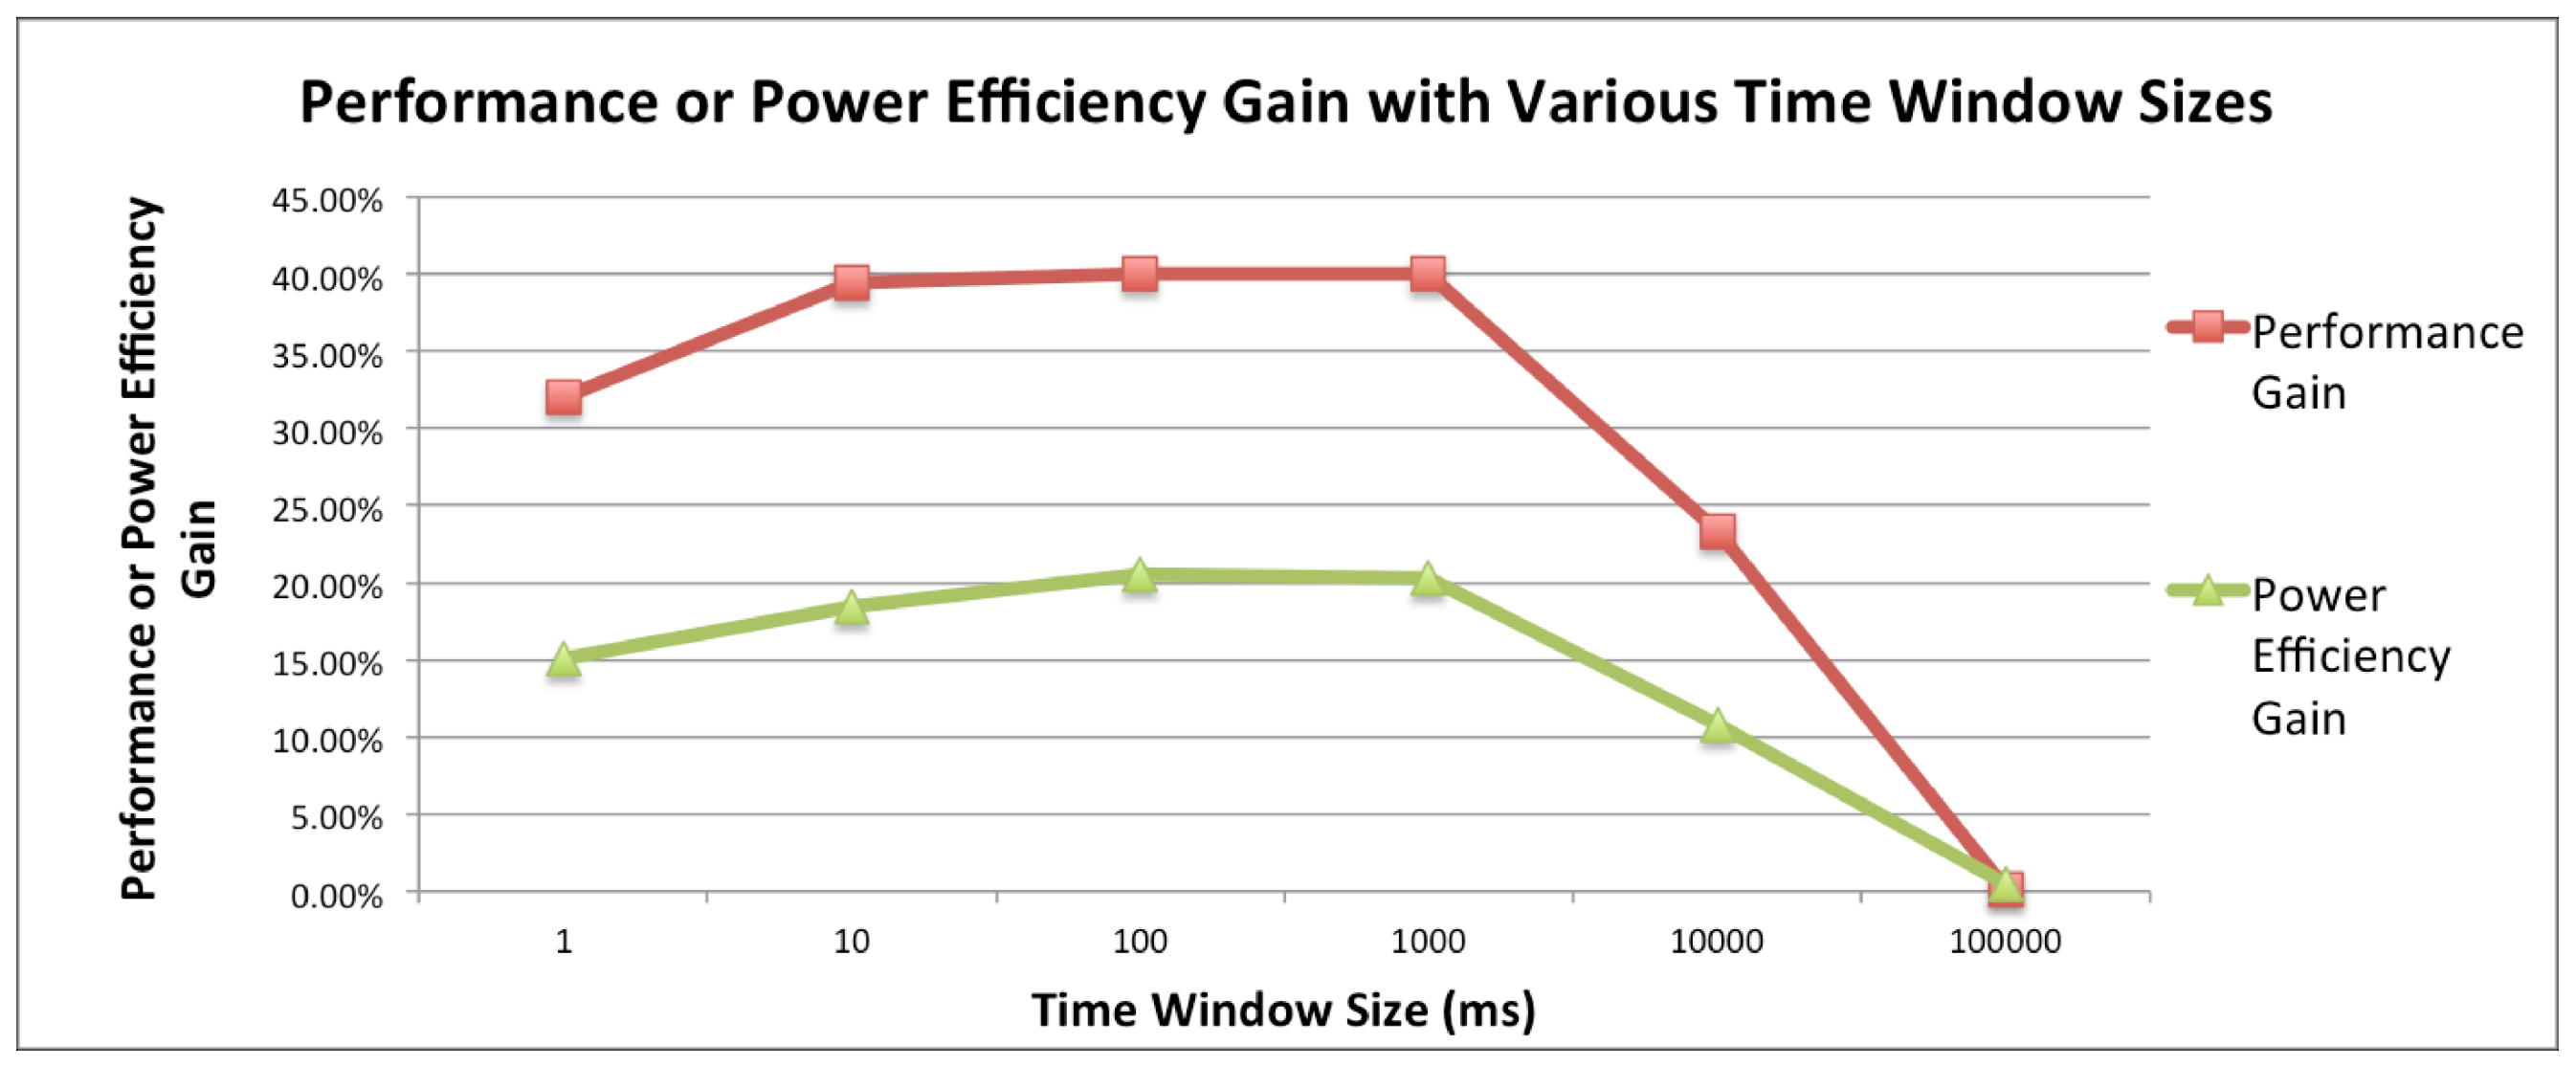
\includegraphics[width=4.5in]{Time-Window-Size}
    \caption{Performance and Power Analysis with Various Time Window Sizes}
    \label{fig_time_window}
\end{figure}

\subsubsection{Impact of Accelerator Scheduling on Memory-bound vs CPU-bound Applications}

We study the impact of the two scheduling heuristics, bandwidth-first
and speedup-first, for different types of workloads. Furthermore, we compare each of the
heuristics to na\"{\i}ve scheduling, in which case we simply use the calculated priority
rank $P_x$.  We construct two workload bundles based on the memory
access intensity for the benchmarks. The first workload bundle is memory-bound, with a bandwidth of over 500MB/s as shown in 
in Table \ref{tbl_benchmark}. The second workload bundle is CPU-bound.

By design, the
bandwidth-first strategy prioritizes the utilization of memory
bandwidth, which inherently gives benchmarks hungry for memory-bandwidth
more opportunities to take advantage of the accelerator logic. As a result,
this strategy outperforms speedup-first for memory-bound
applications as shown in Figure \ref{fig_mem_bound}. On the other hand,
CPU-bound applications benefit more from the speedup-first
scheduling strategy as depicted in Figure \ref{fig_cpu_bound}.

\begin{figure}
    \centering
    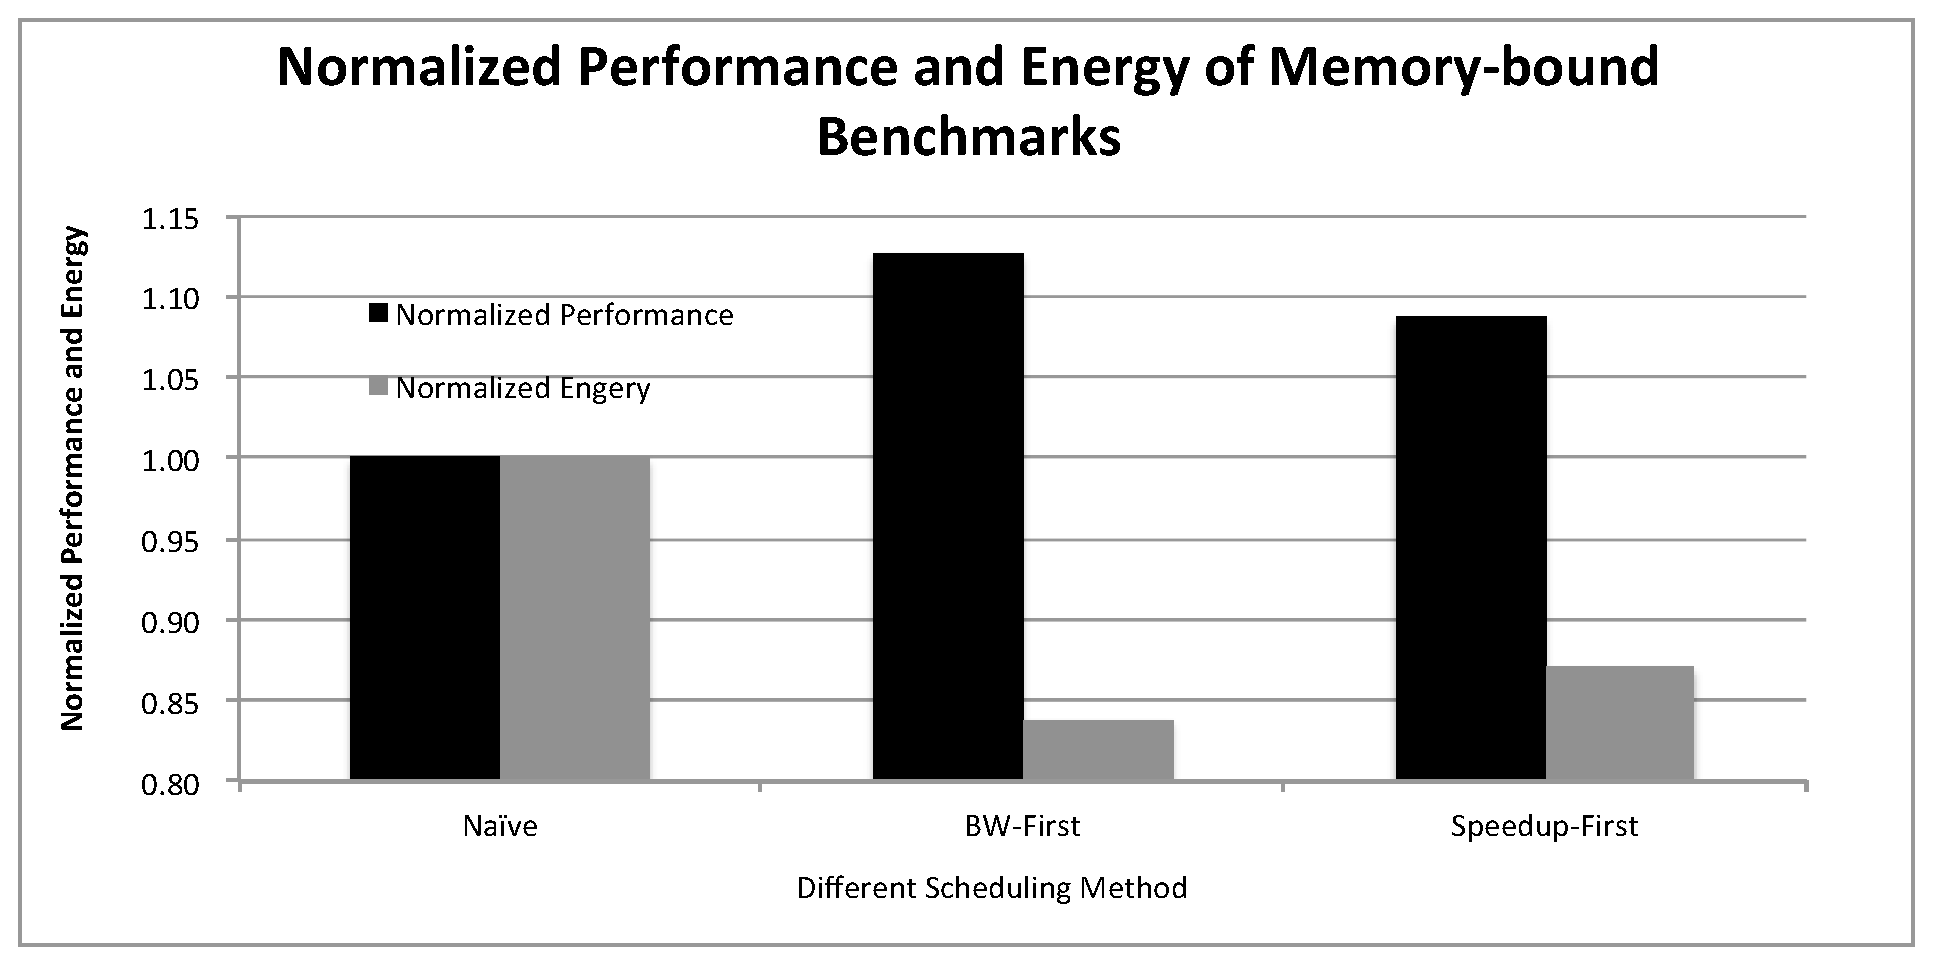
\includegraphics[width=4.5in]{Memory-Bounded}
    \caption{Performance and Energy Consumption of Memory-bound Benchmark Group}
    \label{fig_mem_bound}
\end{figure}

\begin{figure}
    \centering
    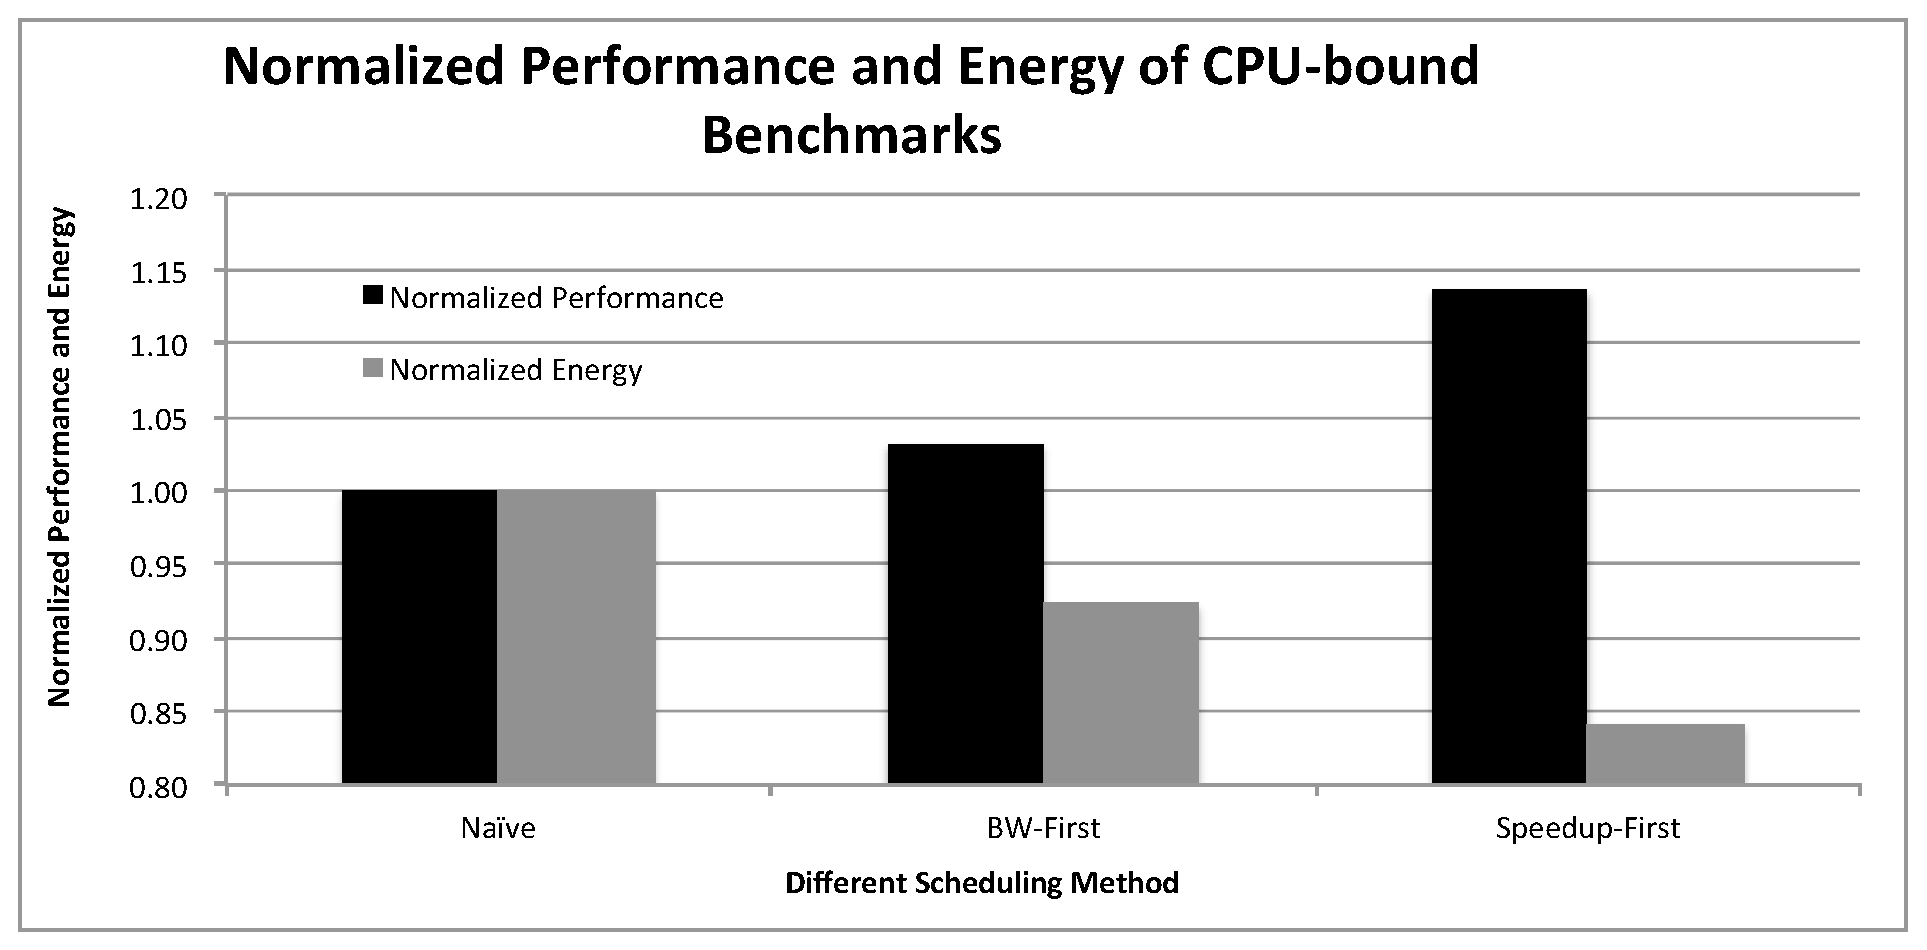
\includegraphics[width=4.5in]{CPU-Bounded}
    \caption{Performance and Energy Consumption on CPU-bound Benchmark Group}
    \label{fig_cpu_bound}
\end{figure}


\subsubsection{Chip Area Allocation}

Given the limited chip area, one particular area of interest is the method utilized for allocating space
 to each of the cores as well as the programmable accelerators.
We vary the number of cores and the size of the
reconfigurable logic to explore the design space. Figure
\ref{fig_core_acc_ratio} was obtained by changing the core and
the accelerator area ratio given a total area equivalent to four cores
as well as a reconfigurable logic unit, which in this case was a default accelerator size similar to the one used
by the Spartan 3E FPGA. As the area of an Atom core is about
    one fourth the size of a Spartan 3E FPGA, the resulting combinations for the cores and the reconfigurable
logic include 8:0, 6:0.5, and so forth. It is interesting to note that the
 5:0.75 ratio produces optimal performance gains while increasing the accelerator
logic continually improves the energy efficiency. While the ratios are
specific to each of the workloads and therefore can only be generalized with caution, 
our results indicate that it is important to
investigate the design space in order to determine the best possible
arrangement for the cores as well as the accelerators. 

\begin{figure}
    \centering
    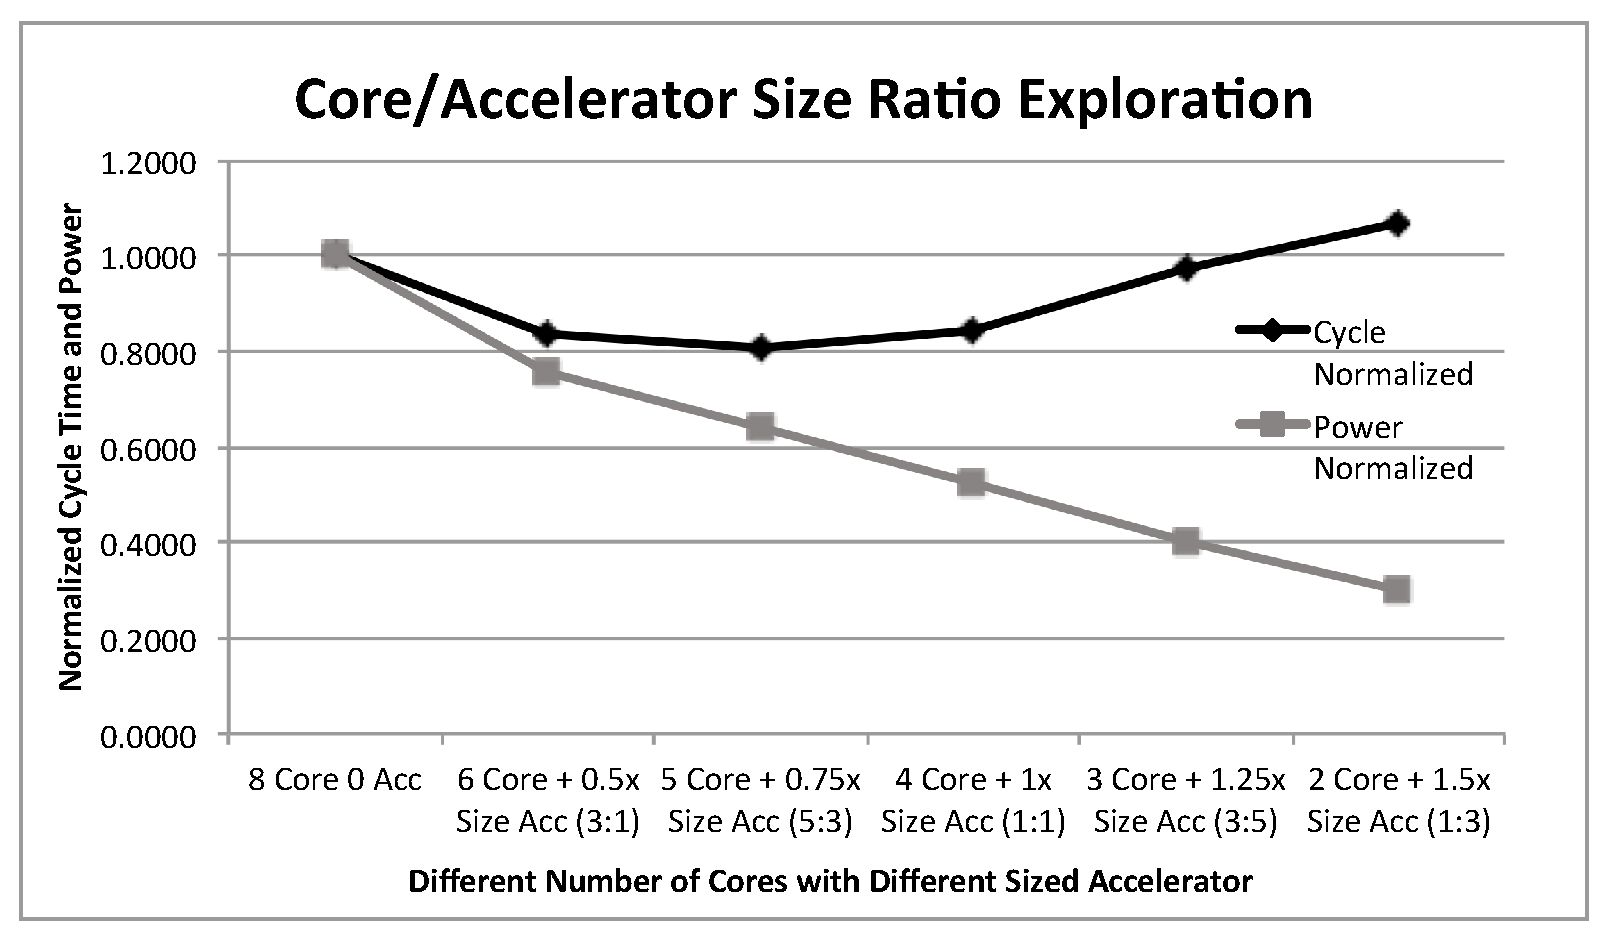
\includegraphics[width=4.5in]{Core-Acc-Size-Ratio}
    \caption{Performance and Power with Different Core/Accelerator Ratios}
    \label{fig_core_acc_ratio}
\end{figure}

\subsubsection{Architectural Parameter Analysis}

One of the contributions of this work is to provide insights into how
different parameters of the heterogeneous architecture or the
benchmark will affect the performance and the power efficiency of the
resulting heterogeneous architecture. Thus, we explore the same performance and
energy efficiency metrics with respect to different architectural parameters in order to
 better understand their implications. 

First, we study the effects of the L1 cache size as shown in Figure \ref{fig_l1_perf}. Our
system consisting of 32 KB of L1 cache employing a na\"{\i}ve scheduling algorithm is considered as the
baseline for this experiment. The performance gain increases rapidly as the
L1 cache size changes from 8 KB to 32 KB, specifically between 12\% to 14\%.
However, the performance gains decrease as the cache size increases beyond 32
KB. The aforementioned findings indicate that 32 KB of L1 cache is sufficiently large
 for our benchmarks. As shown in Figure
\ref{fig_l1_power}, the power efficiency decreases
steadily as the cache size increases. In this case, the increase in the cache size 
tends to significantly increase both the static power as well as the dynamic power. 

We conduct a similar experiment by changing the L2 cache size, displaying
the results in Figure \ref{fig_l2_perf} and \ref{fig_l2_power}. As
we increase the size of the L2 cache, the performance gain increases while the
power efficiency gain steadily decreases. However, the slope of the gain is significantly larger by comparison with the results obtained for 
the L1 cache. In this case, the accelerators and the CPUs share the L2 cache with the MOESI coherence. As a result, when the cache size 
increases, the heterogeneous architecture benefits from the lower cache miss rate. 

The accelerator's local buffer works in similar manner to the core's L1 cache. Thus, the characteristics of the accelerator local buffer 
resemble the characteristics of the L1 cache as shown in Figure \ref{fig_acc_buffer_perf} and \ref{fig_acc_buffer_power}. 
The only difference is that as we adjust the buffer size, the rate of change for the gains of the local buffer is larger 
by comparison with the L1 cache. In this case the hardware implementation is more sensitive to the locality of the input data
 given that there is a higher level of data parallelism within the accelerators. 

We also study the inter-arrival time of the Poisson-distributed benchmark mixture to find if the dynamics of the workload will affect 
system performance. As illustrated in Figure \ref{fig_benchmark-switching}, we take the 500 million cycles inter-arrival time with na\"{\i}ve
 scheduling as the baseline since ``500 million cycles" is the setup in our experiment. The performance gain tends to decrease as 
the benchmark inter-arrival time varies from 0 cycles to 1000 million cycles. When the inter-arrival time is set to 0 cycles, it becomes
 identical to the continuously arriving back-to-back workload. This figure demonstrates that the more frequent the change in the workload of 
the benchmarks, the more precise the profiling-prediction, and the larger the gains from the scheduling methods. The aforementioned gains
are realized in spite of the increasing overhead due to accelerator reprogramming. In addition, as the inter-arrival time increases, 
the difference in the performance gains increases when comparing the na\"{\i}ve scheduling methods with the other two methods. 
In this case, the benefits of prediction decrease as the inter-arrival time becomes significantly large. However, both the bandwidth-first and
 the speedup-first scheduling algorithms benefit from accelerator combination. 

\begin{figure}
    \centering
    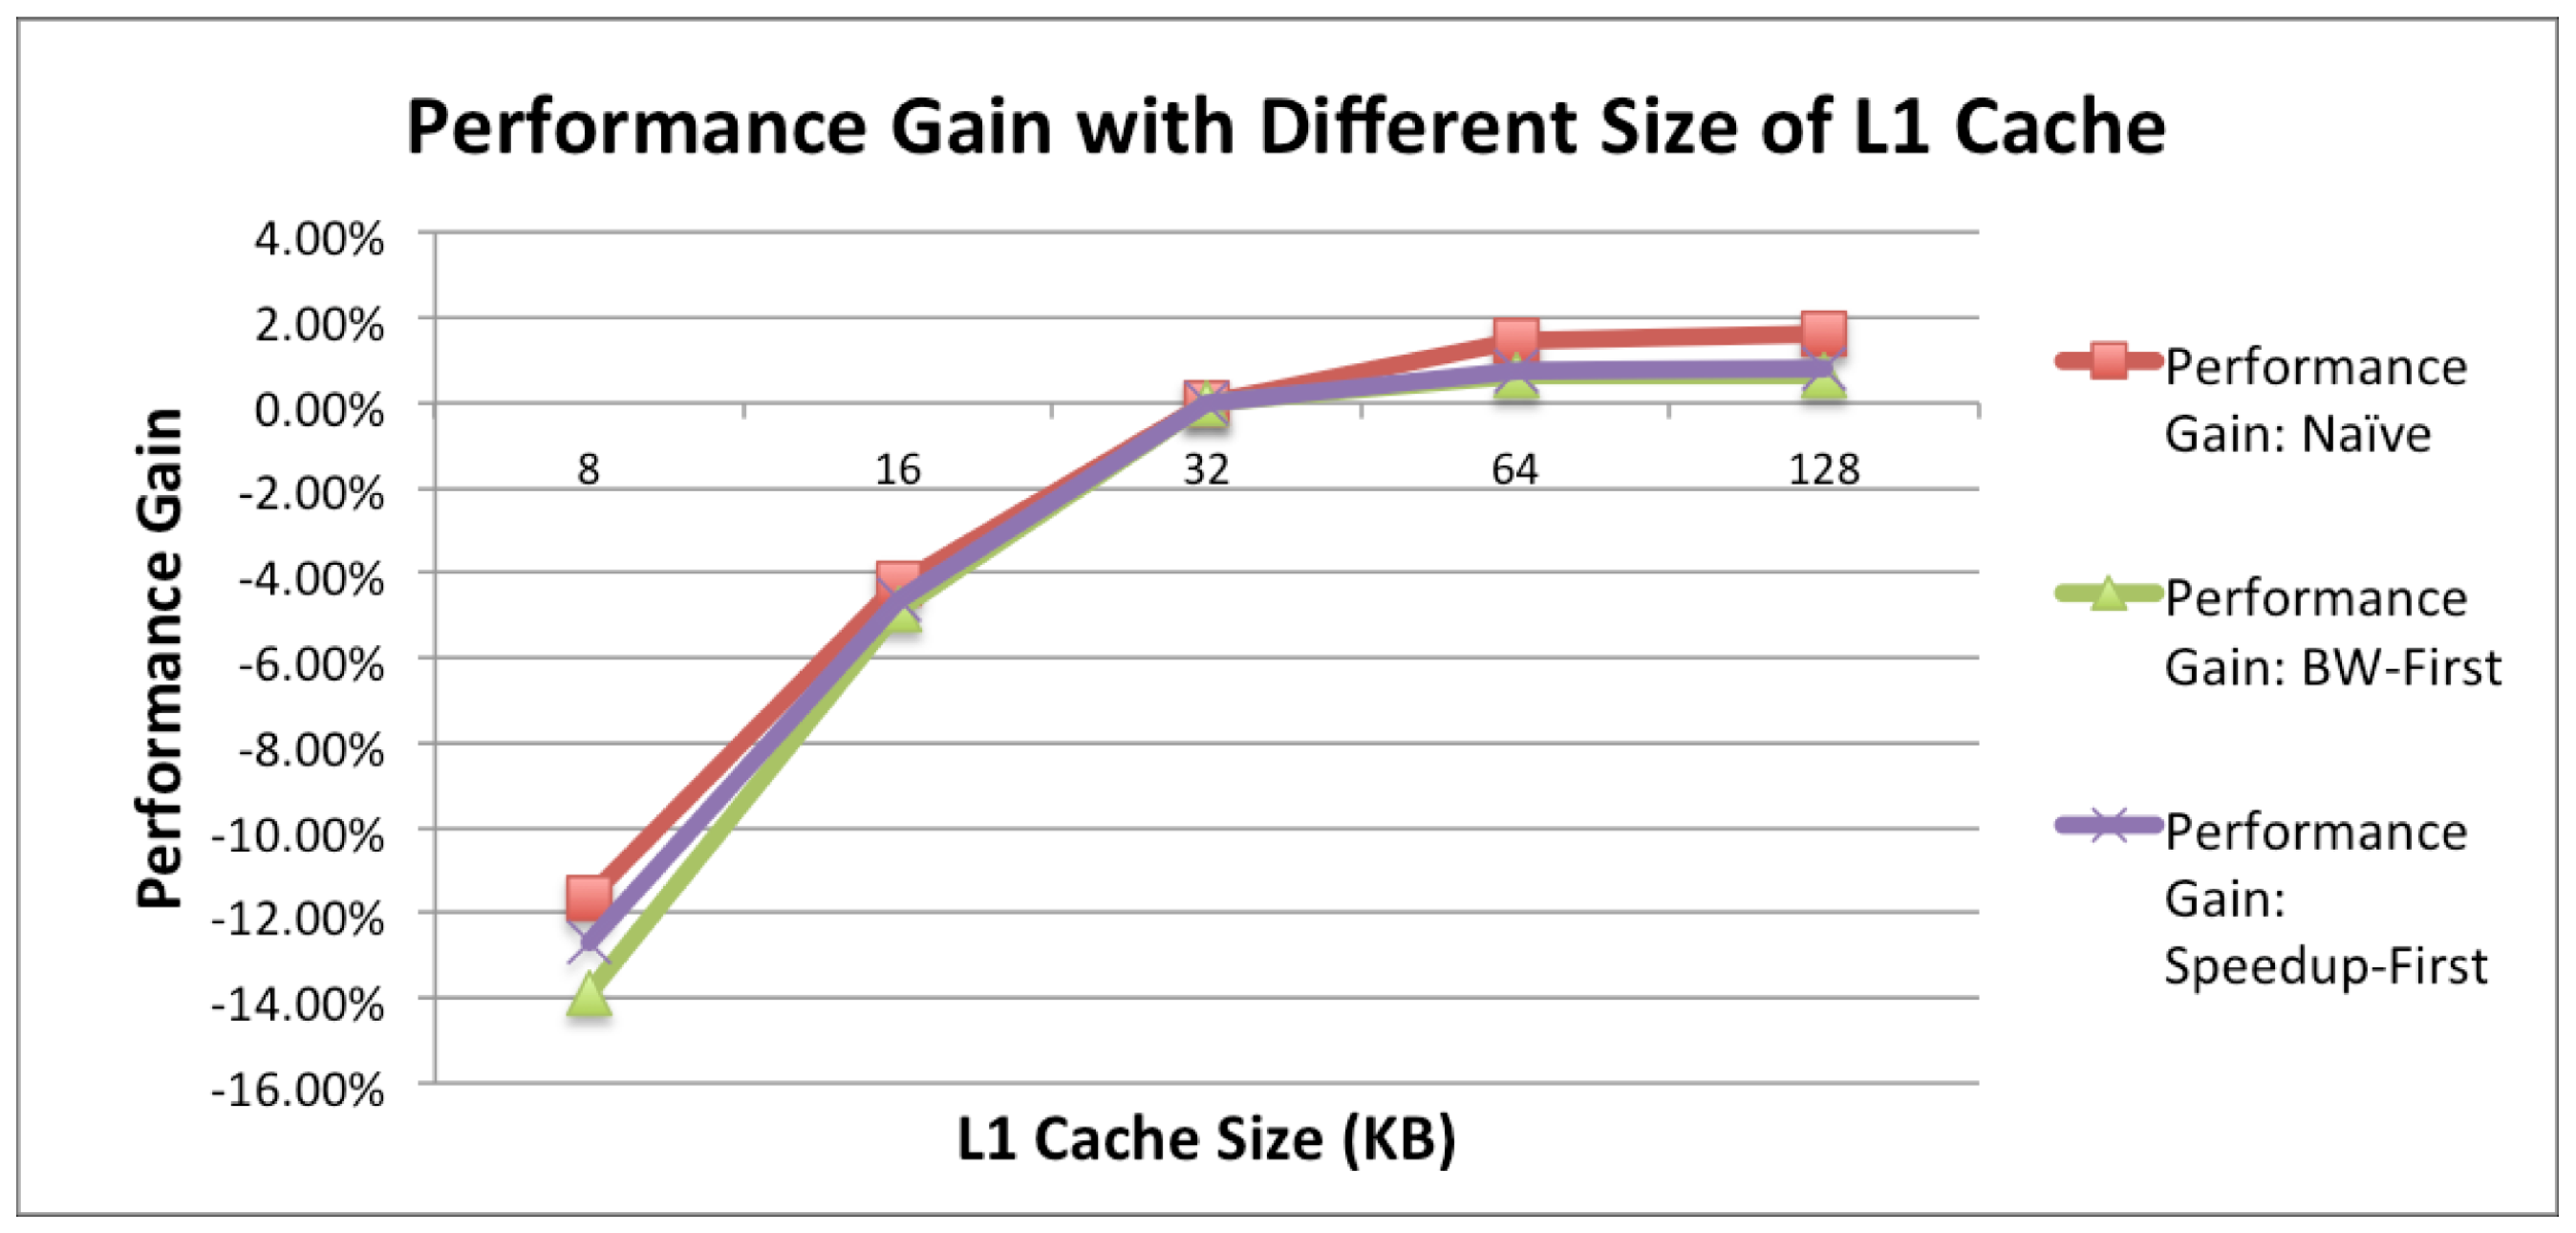
\includegraphics[width=4.5in]{L1-Cache-Performance}
    \caption{Performance Gain with Different Sizes of L1 Cache}
    \label{fig_l1_perf}
\end{figure}

\begin{figure}
    \centering
    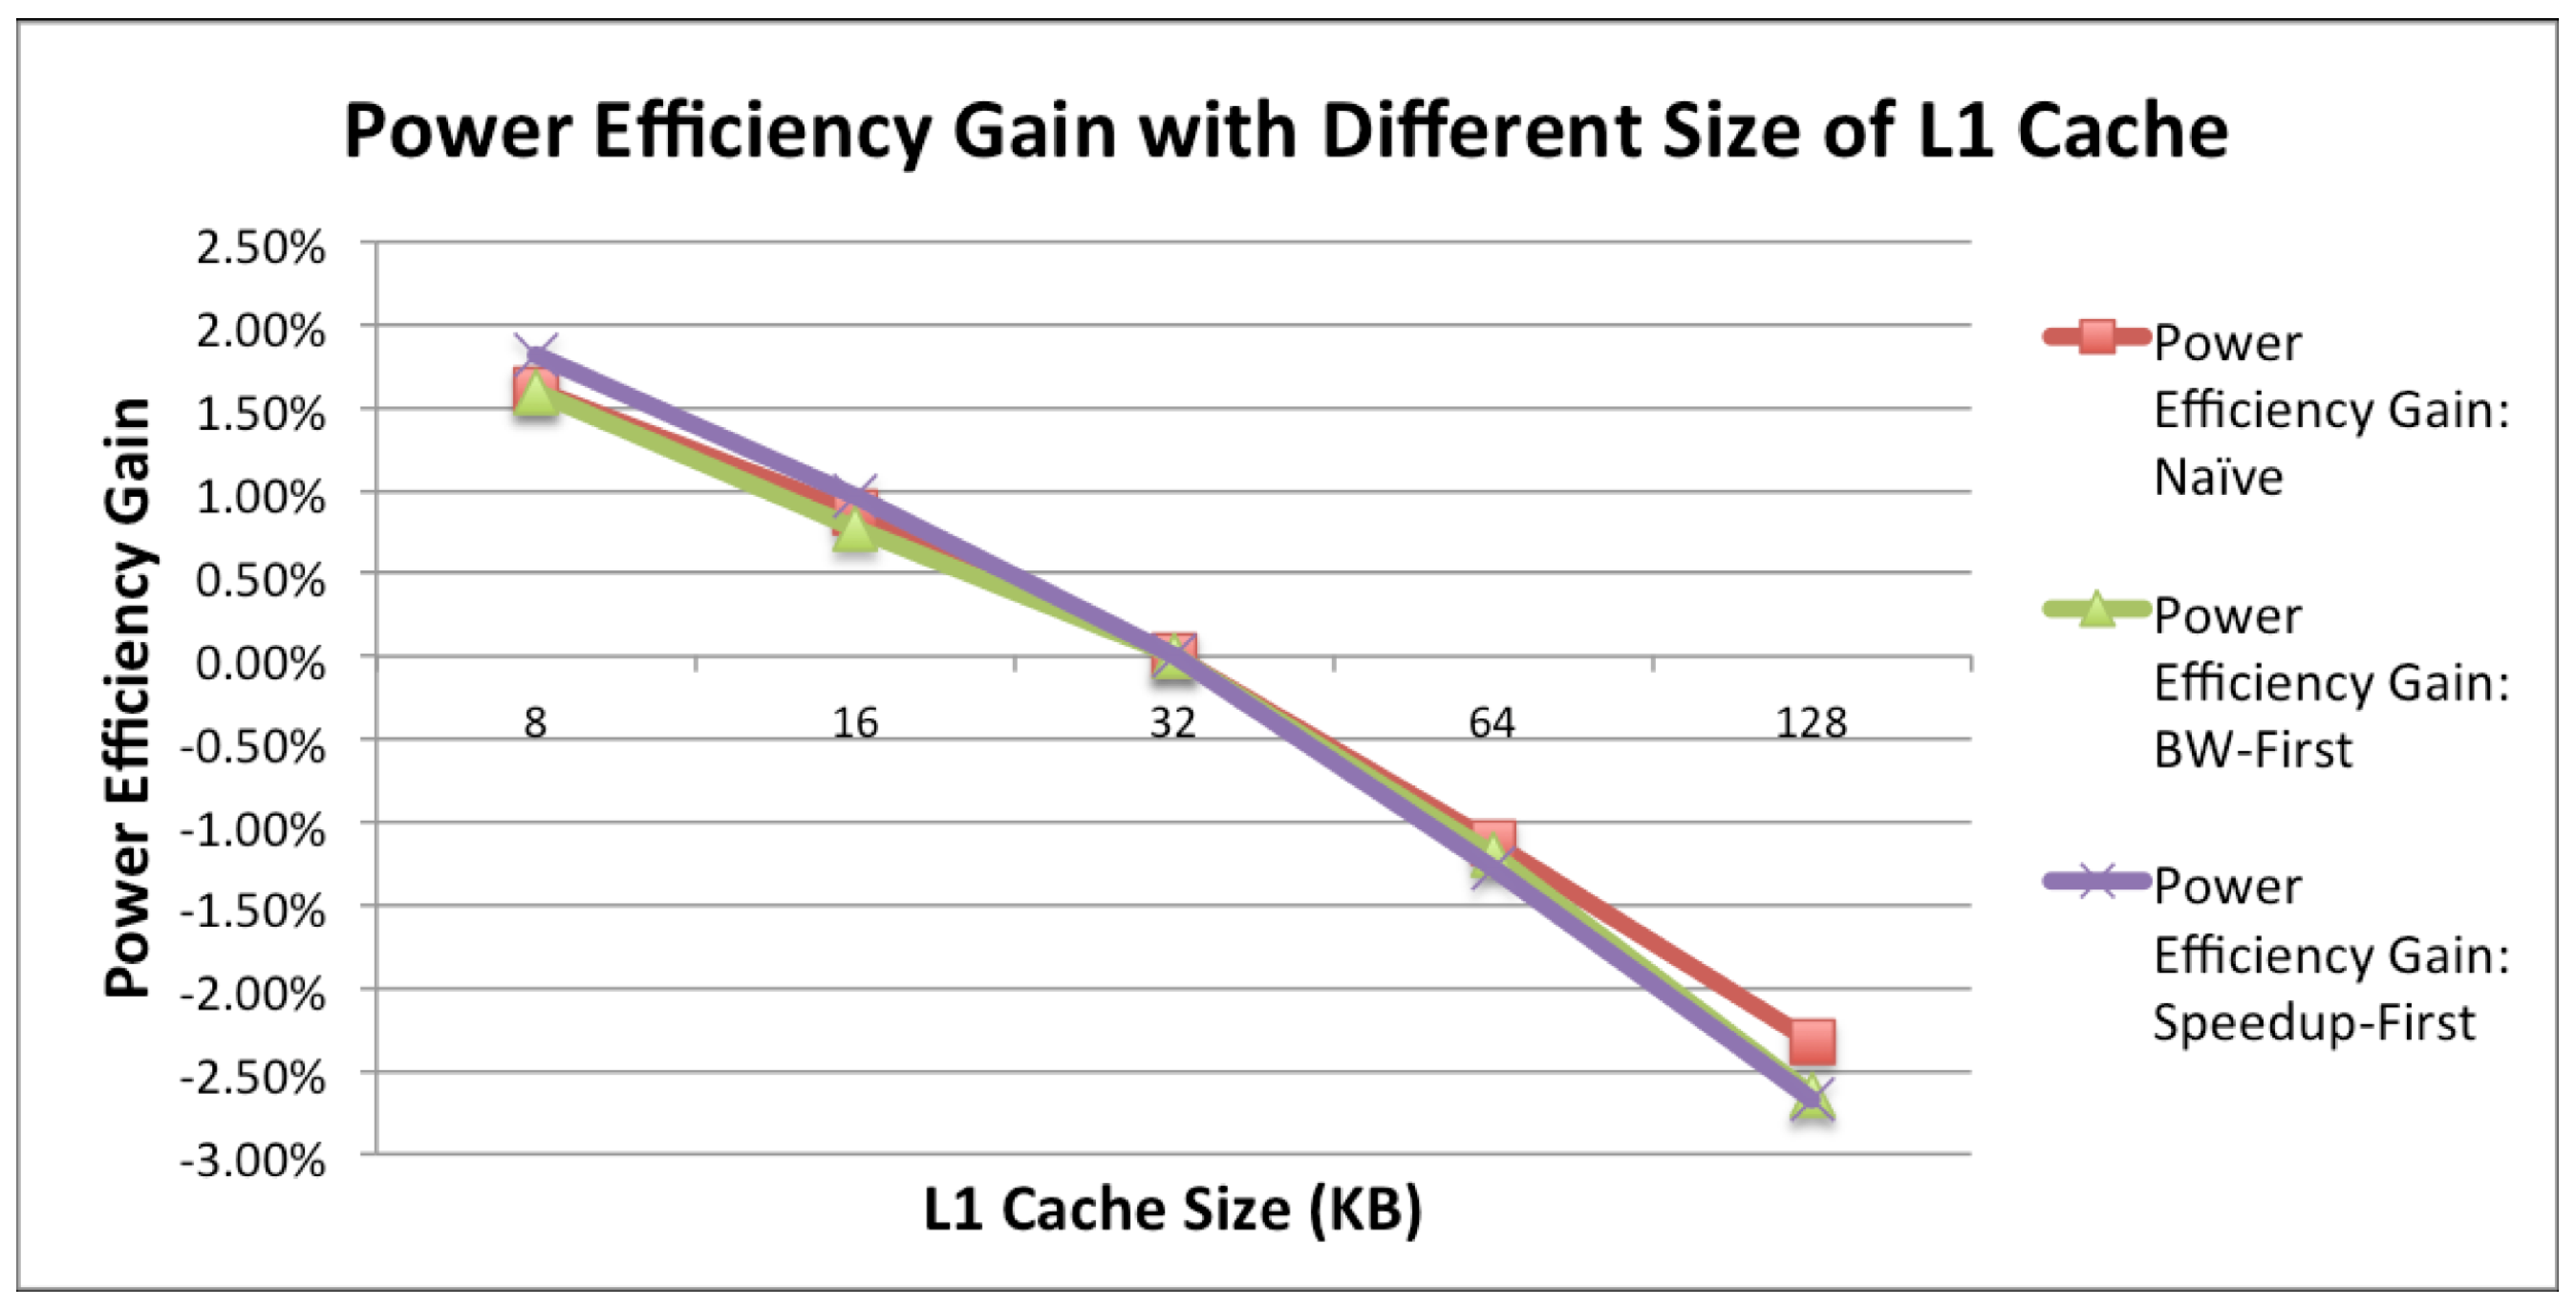
\includegraphics[width=4.5in]{L1-Cache-Power}
    \caption{Power Efficiency Gain with Different Sizes of L1 Cache}
    \label{fig_l1_power}
\end{figure}

\begin{figure}
    \centering
    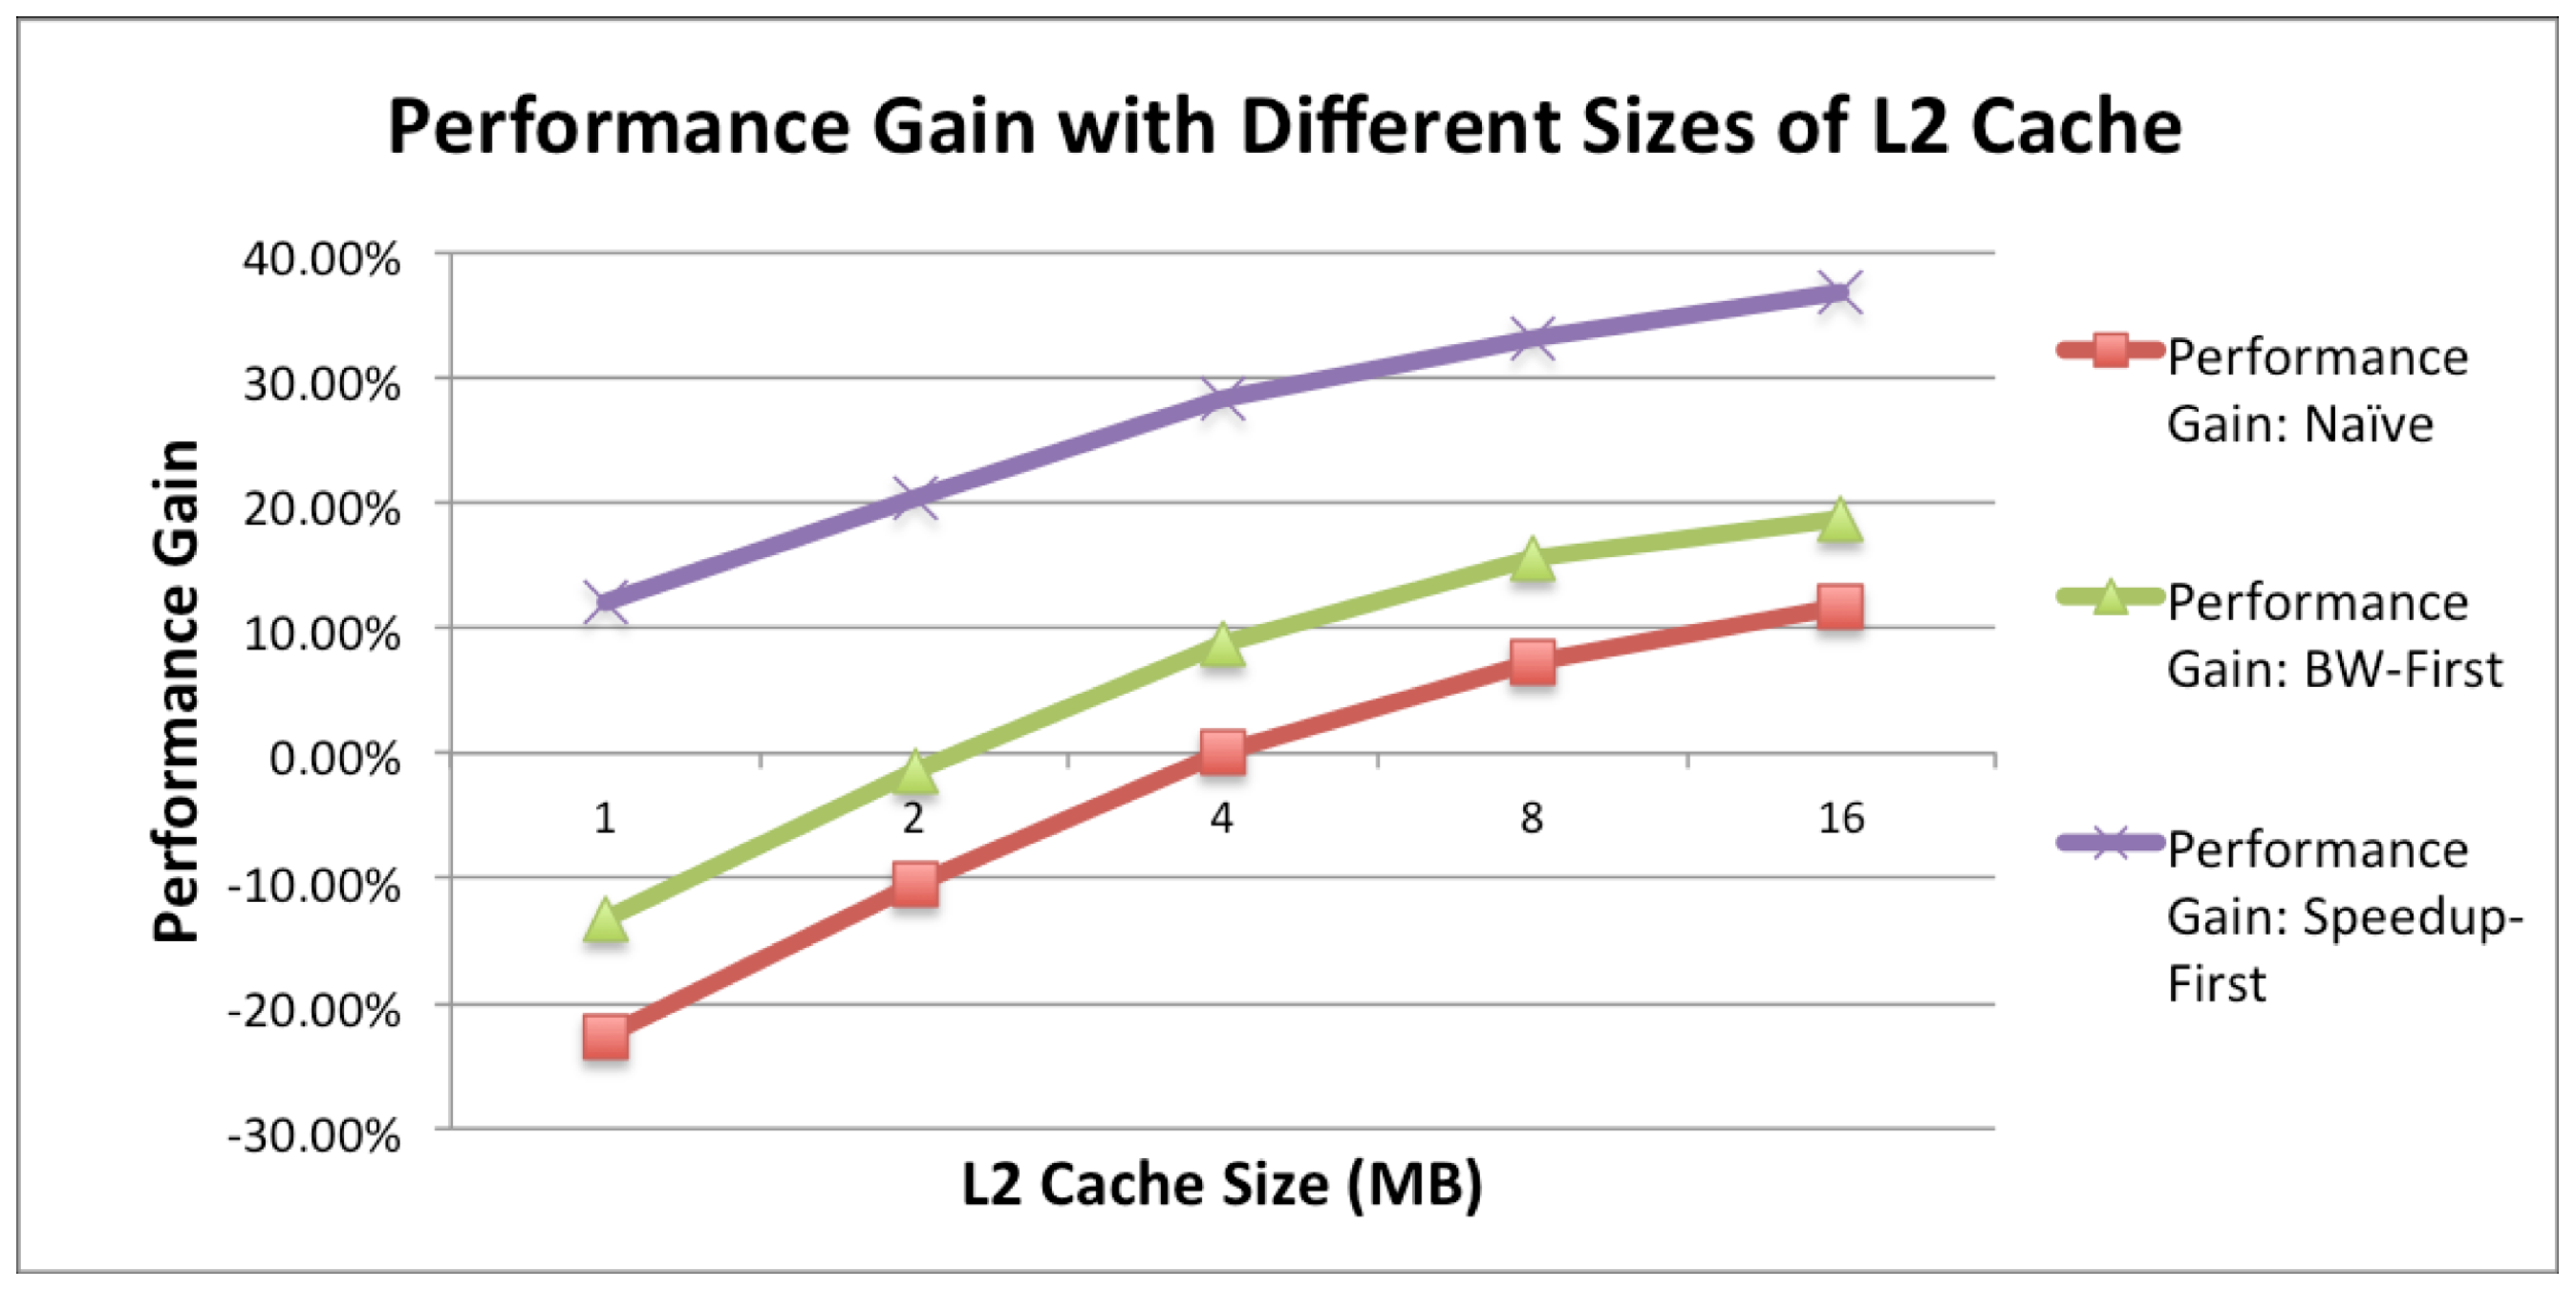
\includegraphics[width=4.5in]{L2-Cache-Performance}
    \caption{Performance Gain with Different Sizes of L2 Cache}
    \label{fig_l2_perf}
\end{figure}

\begin{figure}
    \centering
    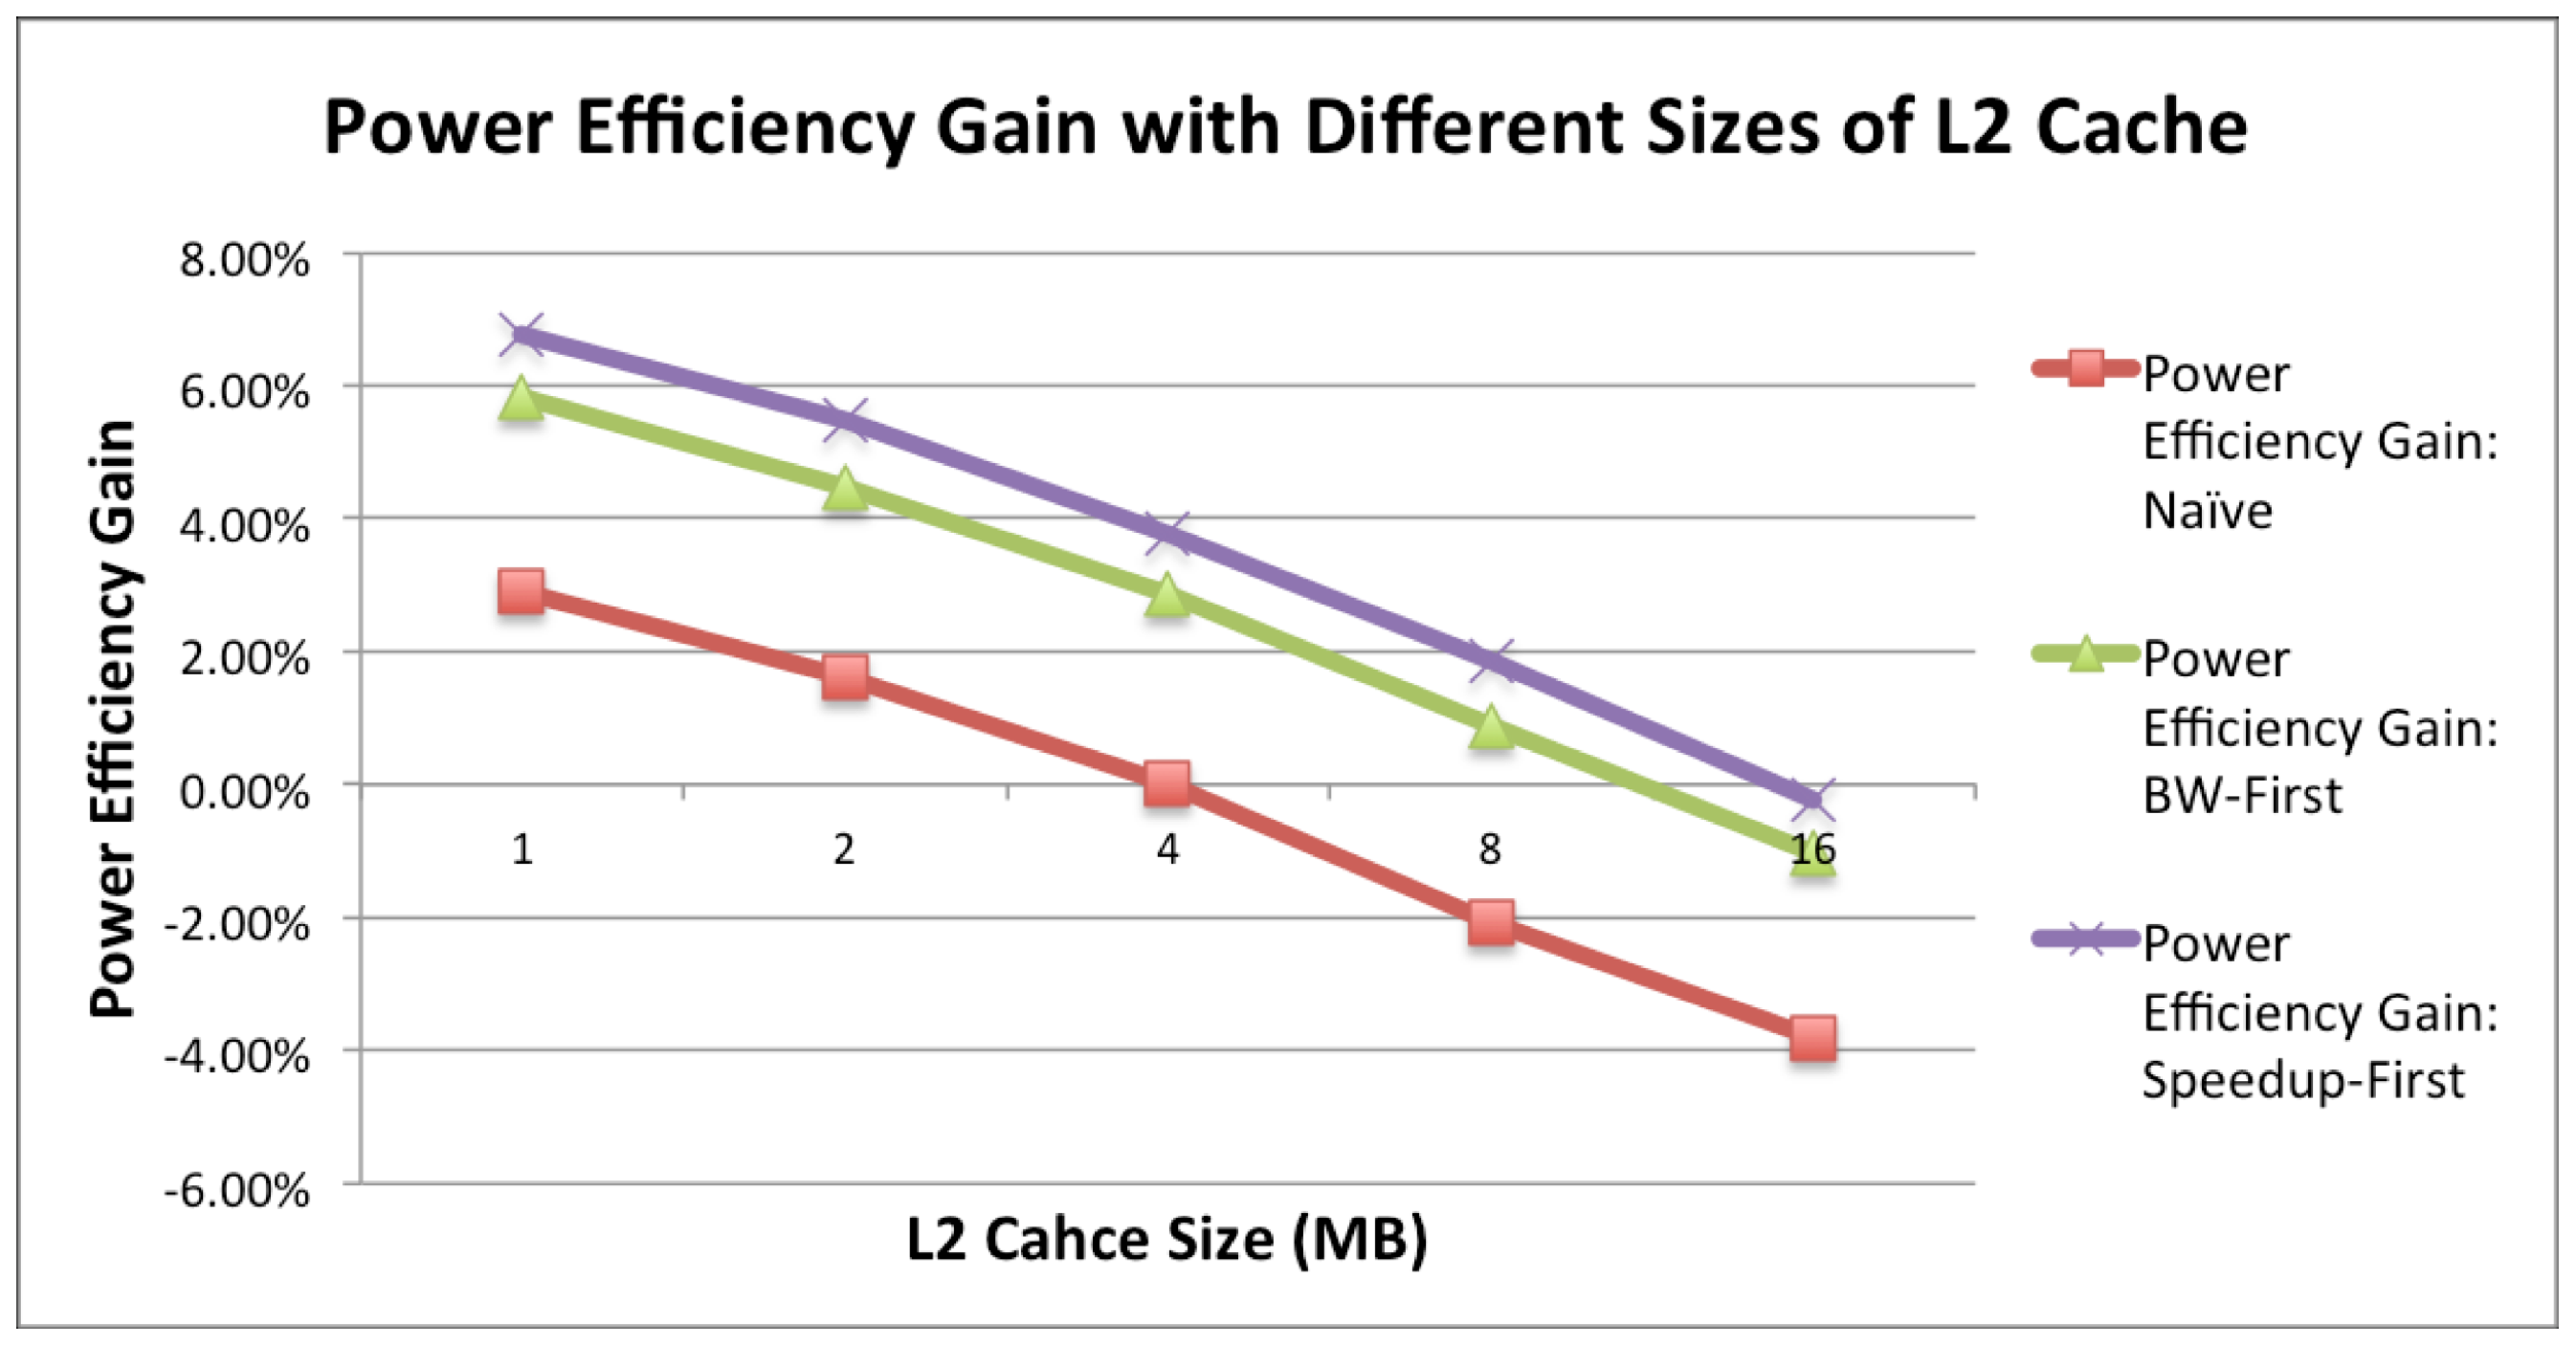
\includegraphics[width=4.5in]{L2-Cache-Power}
    \caption{Power Efficiency Gain with Different Sizes of L2 Cache}
    \label{fig_l2_power}
\end{figure}

\begin{figure}
    \centering
    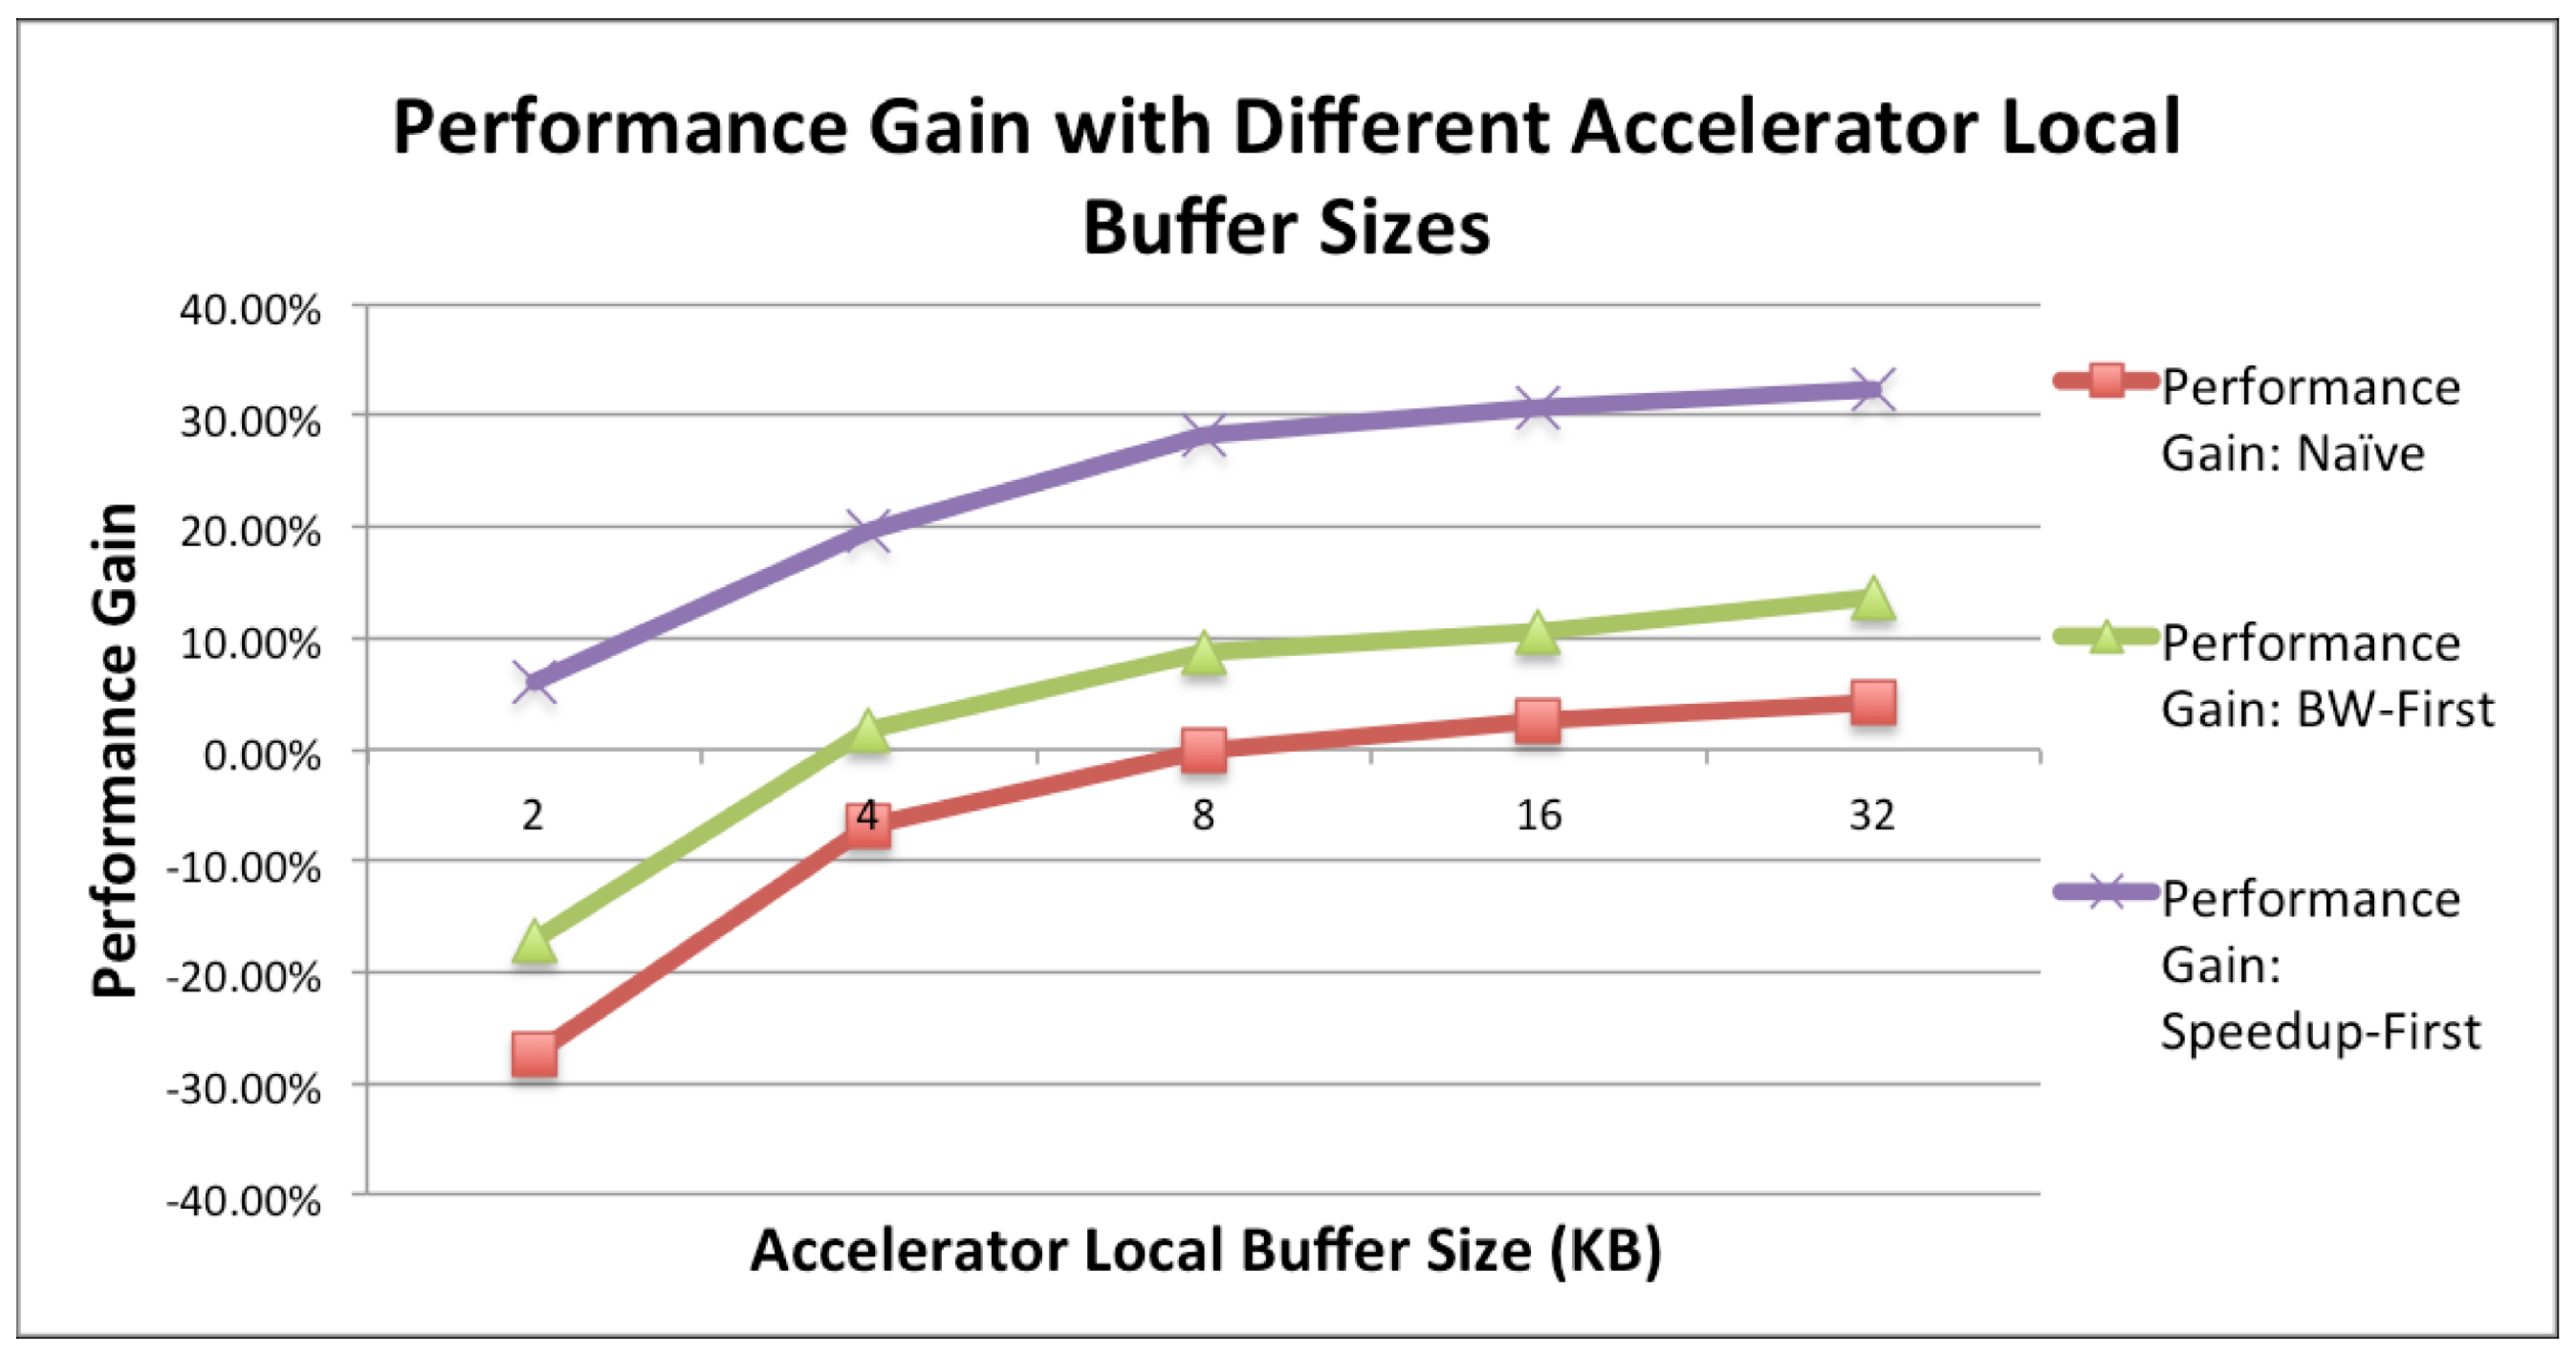
\includegraphics[width=4.5in]{Acc-Buffer-Performance}
    \caption{Performance Gain with Different Sizes of Accelerator Local Buffer}
    \label{fig_acc_buffer_perf}
\end{figure}

\begin{figure}
    \centering
    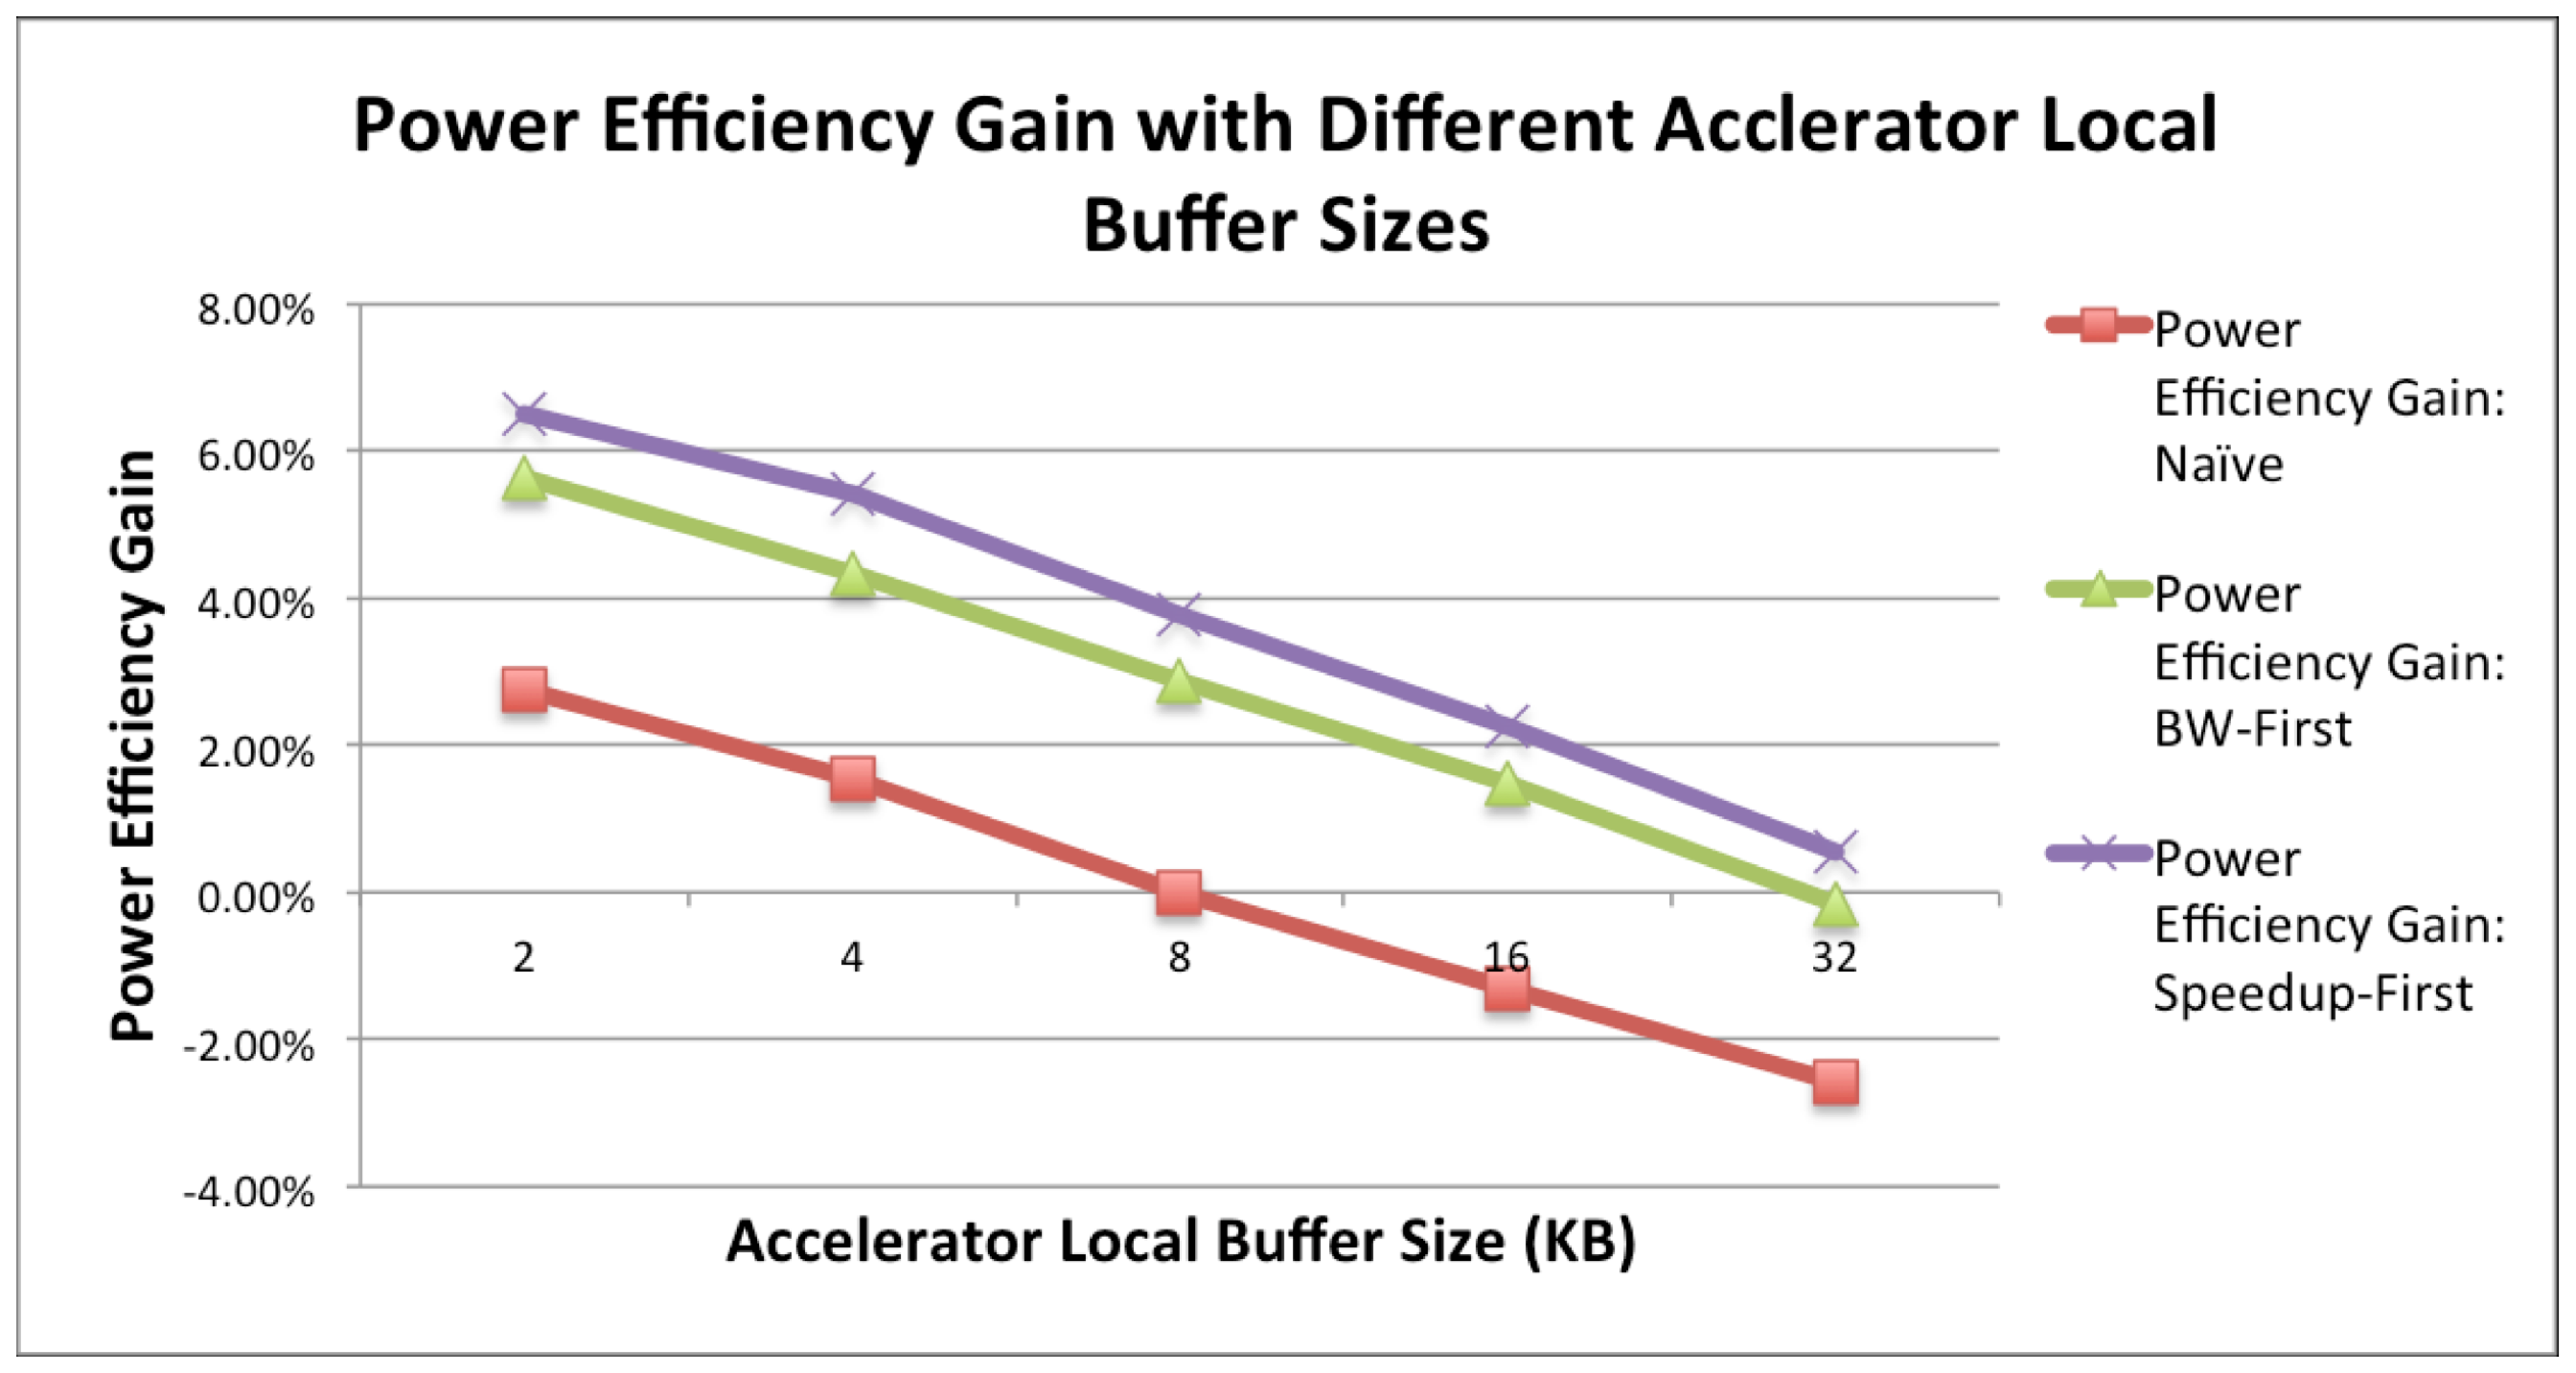
\includegraphics[width=4.5in]{Acc-Buffer-Power}
    \caption{Power Efficiency Gain with Different Sizes of Accelerator Local Buffer}
    \label{fig_acc_buffer_power}
\end{figure}

\begin{figure}
    \centering
    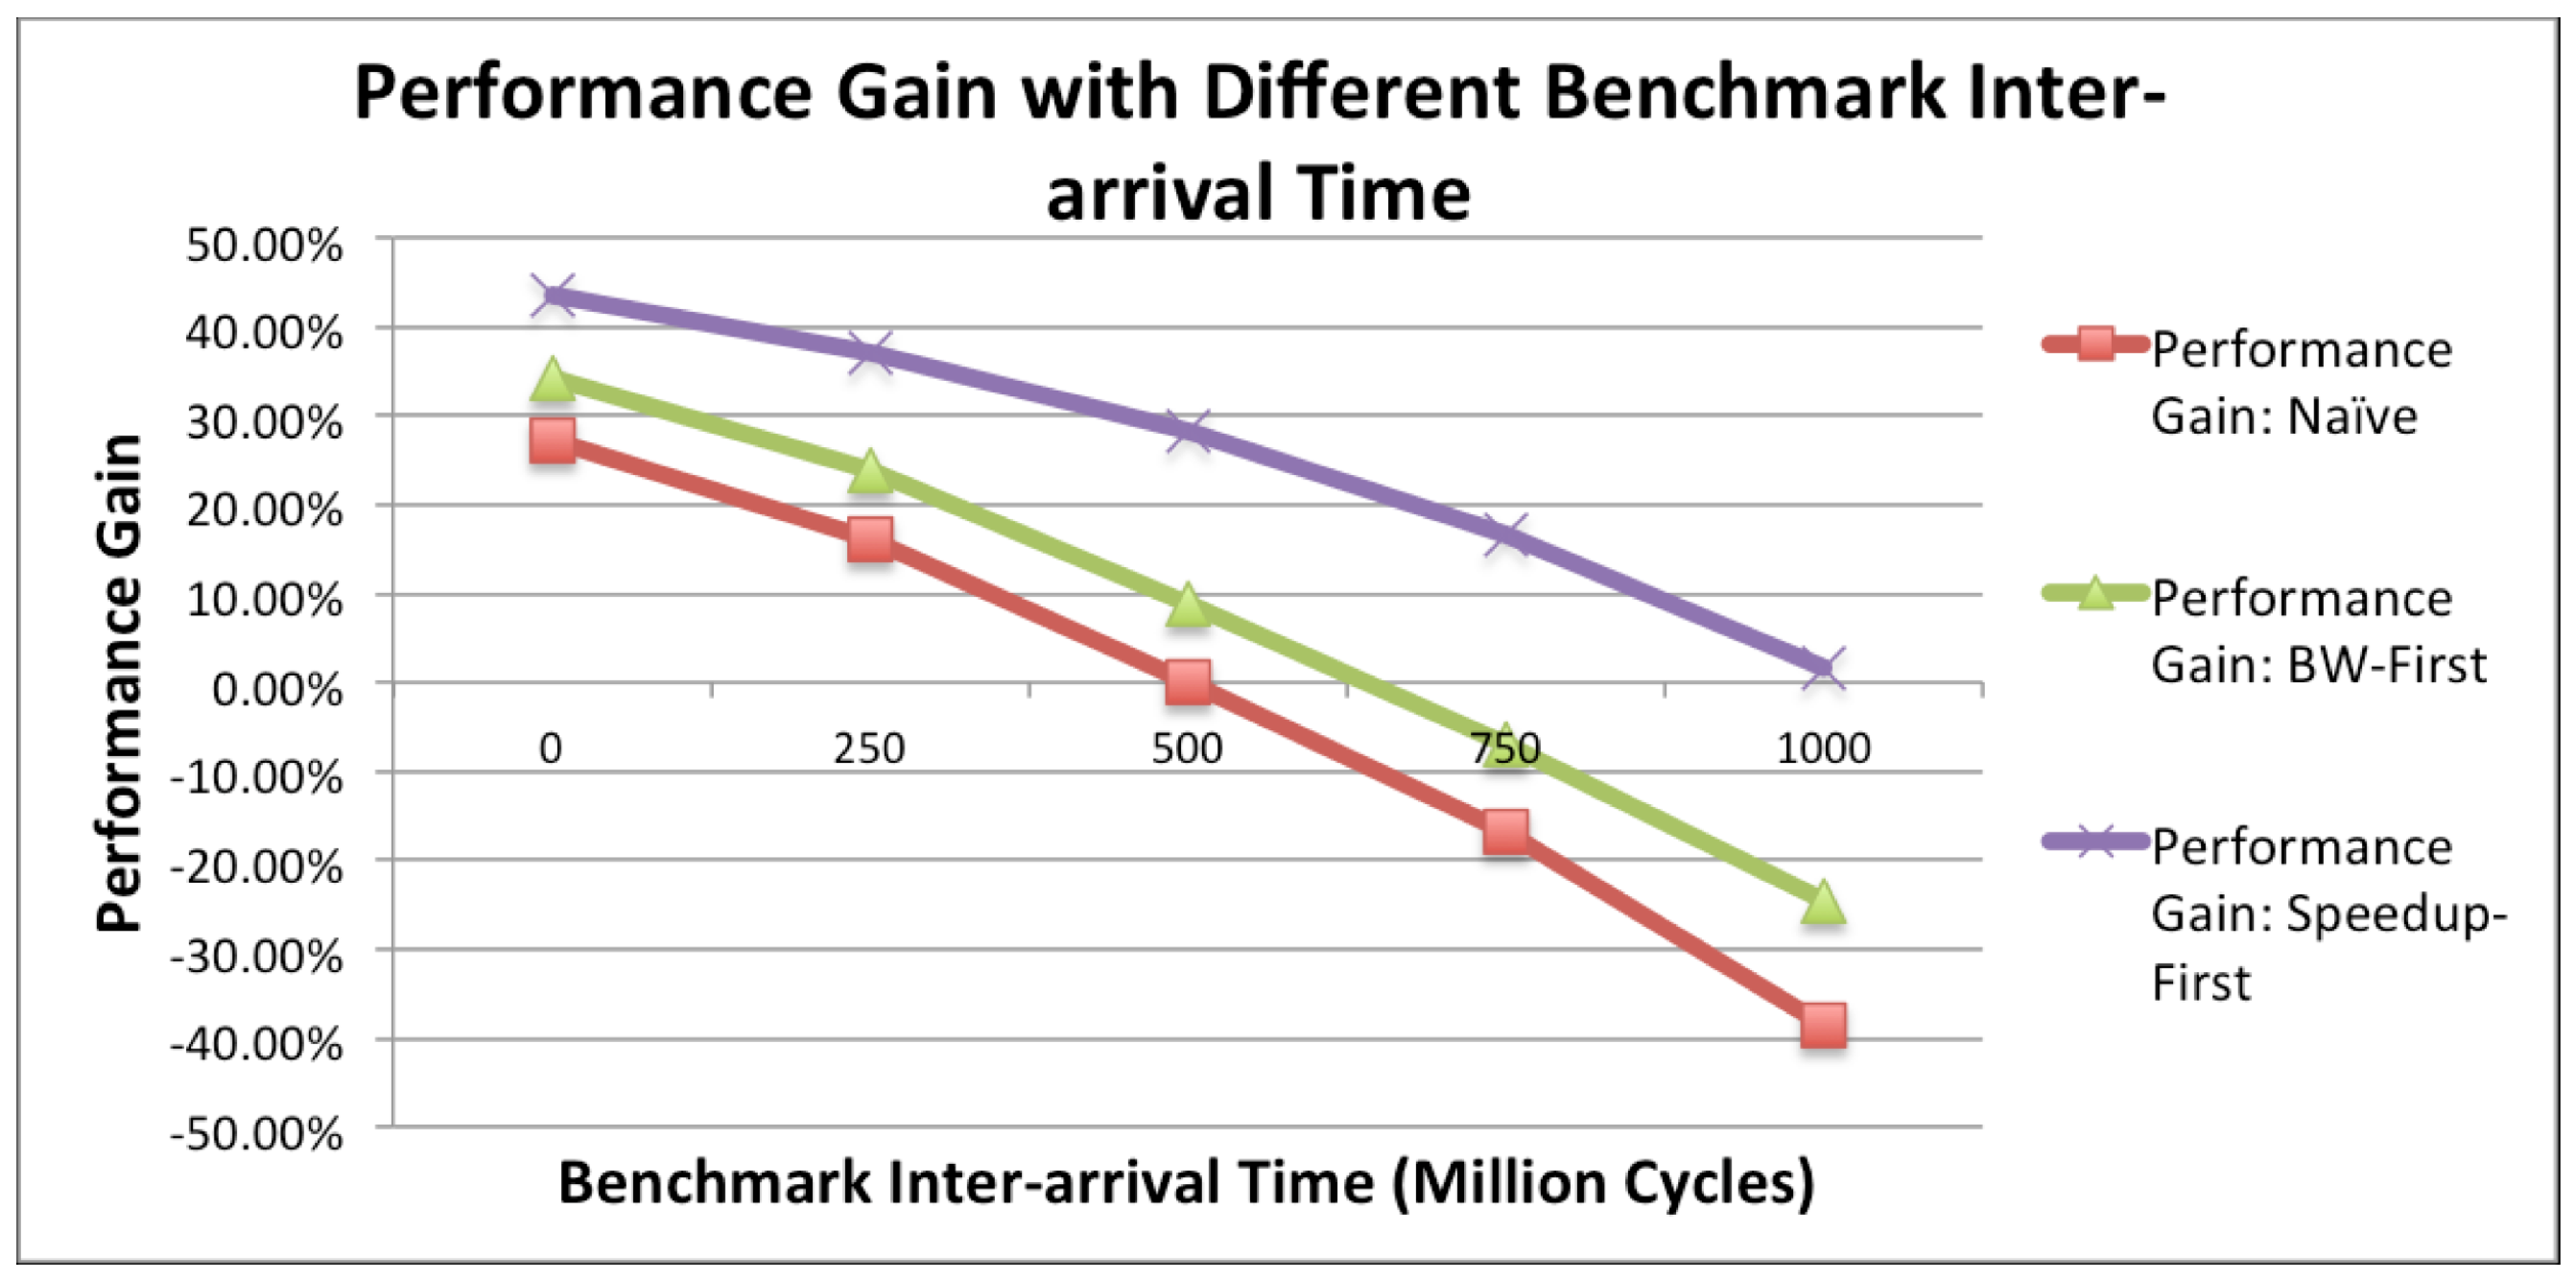
\includegraphics[width=4.5in]{Benchmark-Switching-Time}
    \caption{Performance Gain with Various Benchmark Inter-arrival Time}
    \label{fig_benchmark-switching}
\end{figure}

\subsubsection{Utilization of Reconfigurable Resources}

Figure \ref{fig_acc_timeline} shows a sample of the run-time
reconfiguration process on the {\em Transformer}. The x axis displays the
scheduling time window, while the y axis displays the number of acceleration
functions instantiated on the SoC. Figure \ref{fig_acc_timeline}
reveals the dynamics of the workload and how the {\em Transformer} adapts its
resources to the demanding functions. Figure \ref{fig_logic_timeline}
illustrates how the utilization of various resources within the
reconfigurable logic changes over time.

In addition, Figure \ref{fig_acc_timeline} validates the advantages of using run-time
configuration over fixed accelerators. We make the following observations regarding the maximum number of accelerators. 
The 3DES, SURF, Segmentation, and Smith-waterman functions all resulted in one
instantiation. The IDSI as well as the SLAM-J functions resulted in two instantiations. The SLAM-C as well as Jacobi functions resulted in 
three instantiations. To achieve the same performance relying on the fixed on-chip accelerators, 
the total amount of logic we would need includes: 17,848 SLICE elements, 14,511 FF elements, 13,192 LUT elements, and 255 BRAM elements. 
Specifically, we would need at least 3.8 times
more SLICE elements and 12.75 times more BRAM elements in order to perform comparably with the {\em Transformer}. 
The aforementioned findings serve as an example of the inefficient use of reconfigurable resources.


\begin{figure}[ht]
    \centering
    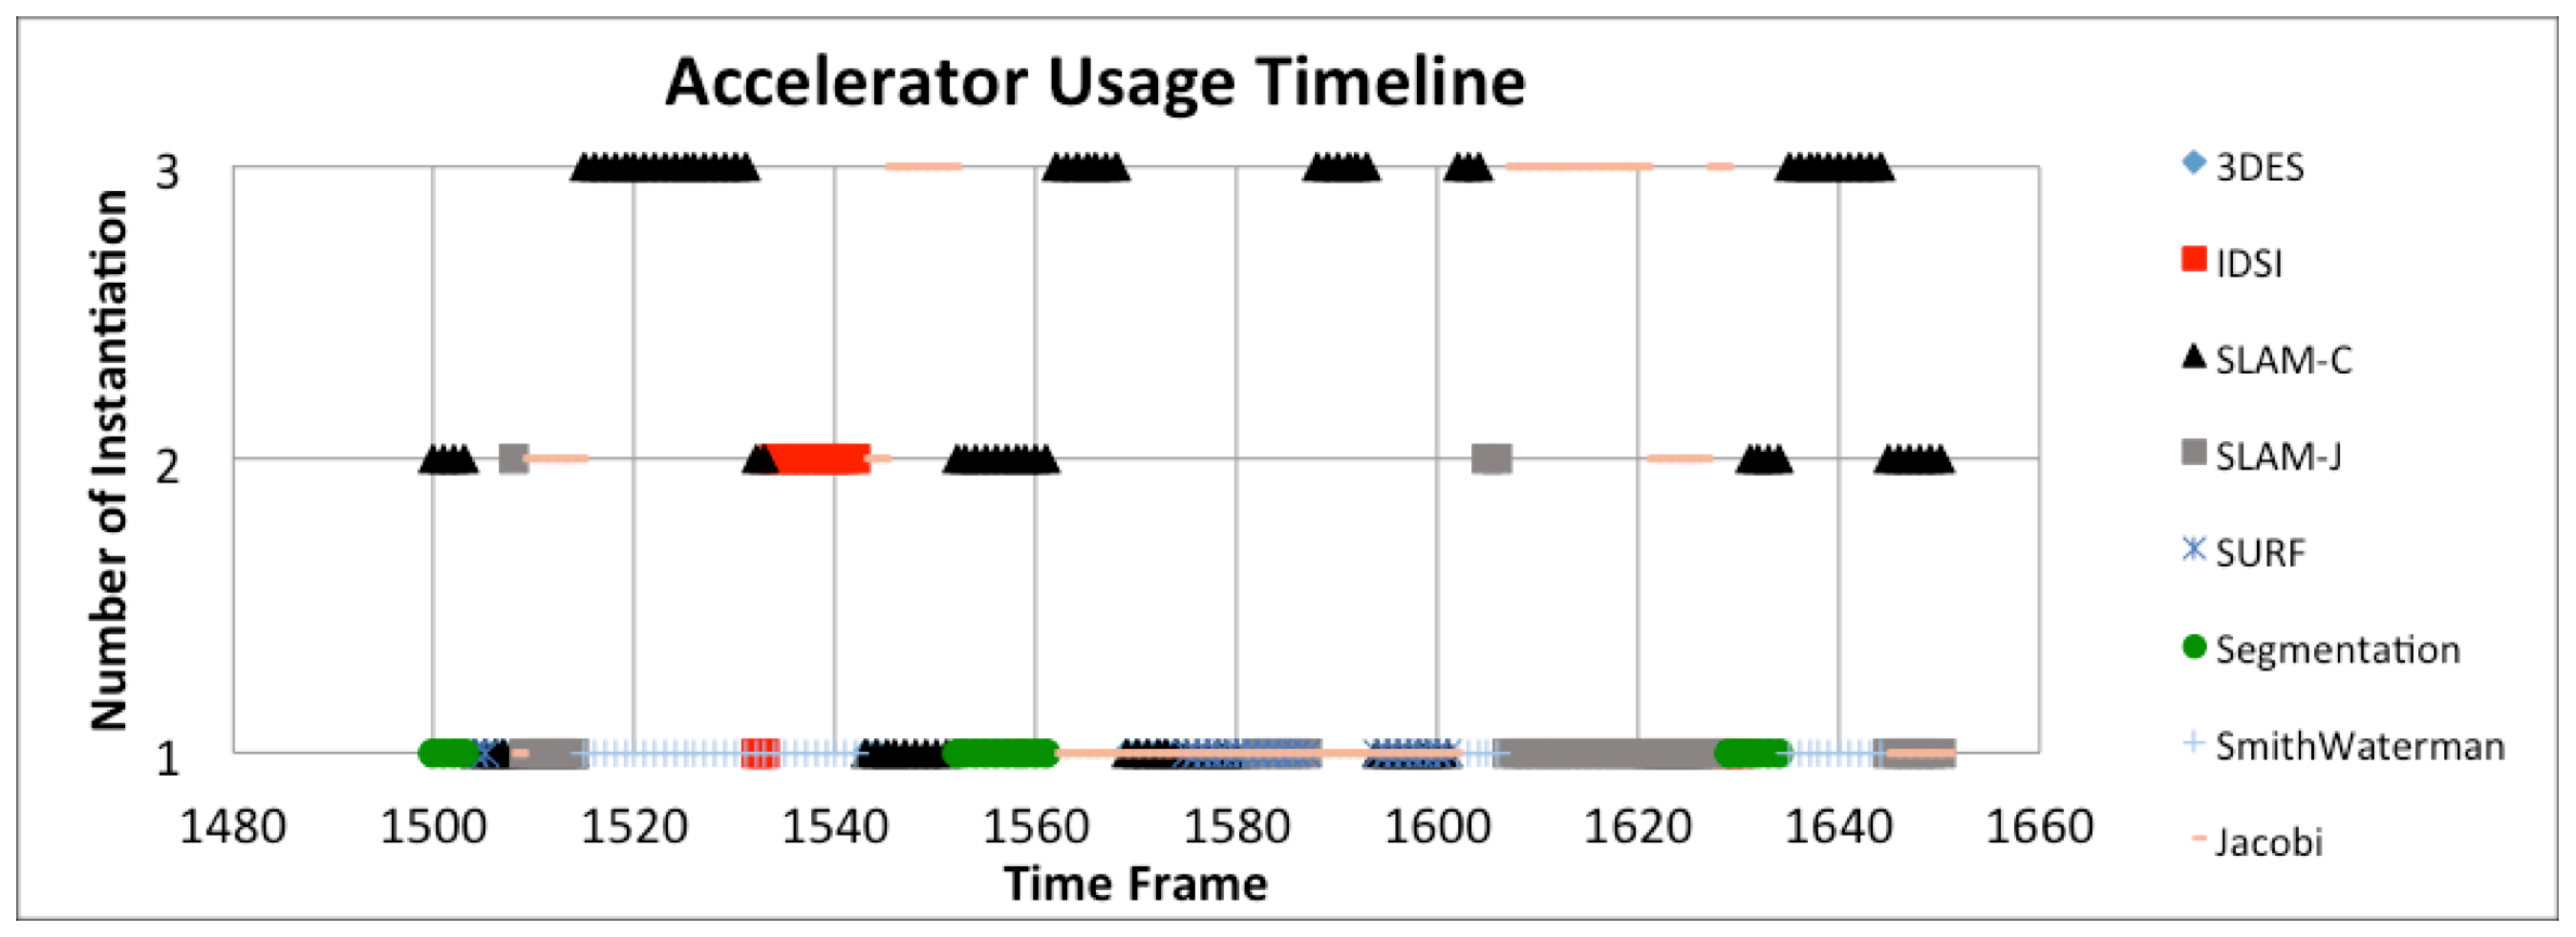
\includegraphics[width=6.0in]{Acc_timeline}
    \caption{Accelerator Usage Timeline}
    \label{fig_acc_timeline}
\end{figure}

\begin{figure}[ht]
    \centering
    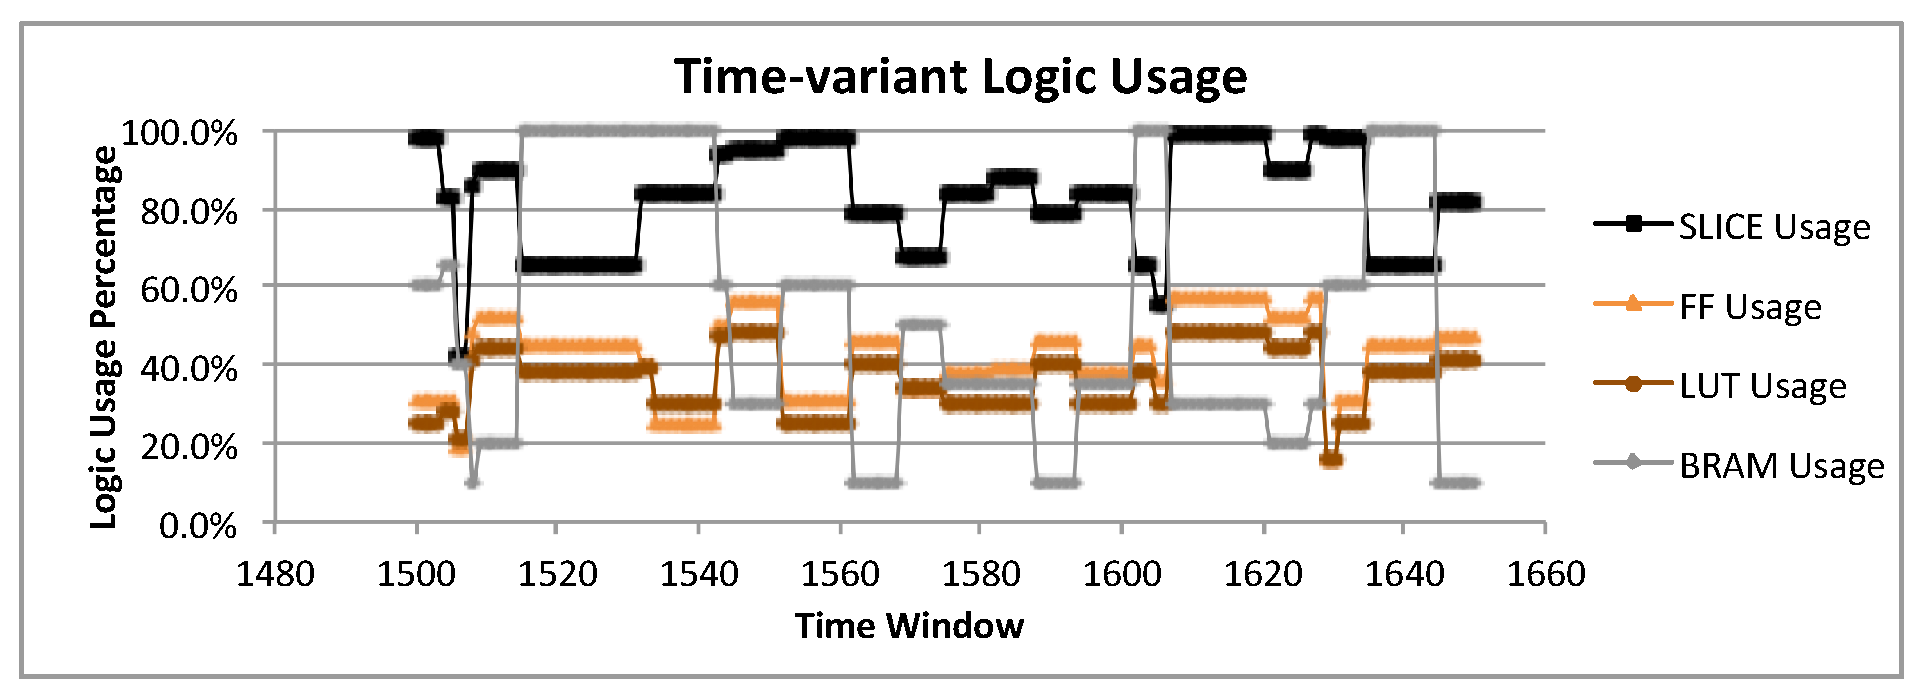
\includegraphics[width=6.0in]{Logic-Usage-Timeline}
    \caption{Total Logic Usage Timeline}
    \label{fig_logic_timeline}
\end{figure}
